% Options for packages loaded elsewhere
\PassOptionsToPackage{unicode}{hyperref}
\PassOptionsToPackage{hyphens}{url}
%
\documentclass[
]{article}
\usepackage{amsmath,amssymb}
\usepackage{lmodern}
\usepackage{iftex}
\ifPDFTeX
  \usepackage[T1]{fontenc}
  \usepackage[utf8]{inputenc}
  \usepackage{textcomp} % provide euro and other symbols
\else % if luatex or xetex
  \usepackage{unicode-math}
  \defaultfontfeatures{Scale=MatchLowercase}
  \defaultfontfeatures[\rmfamily]{Ligatures=TeX,Scale=1}
\fi
% Use upquote if available, for straight quotes in verbatim environments
\IfFileExists{upquote.sty}{\usepackage{upquote}}{}
\IfFileExists{microtype.sty}{% use microtype if available
  \usepackage[]{microtype}
  \UseMicrotypeSet[protrusion]{basicmath} % disable protrusion for tt fonts
}{}
\makeatletter
\@ifundefined{KOMAClassName}{% if non-KOMA class
  \IfFileExists{parskip.sty}{%
    \usepackage{parskip}
  }{% else
    \setlength{\parindent}{0pt}
    \setlength{\parskip}{6pt plus 2pt minus 1pt}}
}{% if KOMA class
  \KOMAoptions{parskip=half}}
\makeatother
\usepackage{xcolor}
\IfFileExists{xurl.sty}{\usepackage{xurl}}{} % add URL line breaks if available
\IfFileExists{bookmark.sty}{\usepackage{bookmark}}{\usepackage{hyperref}}
\hypersetup{
  hidelinks,
  pdfcreator={LaTeX via pandoc}}
\urlstyle{same} % disable monospaced font for URLs
\usepackage[margin=1in]{geometry}
\usepackage{longtable,booktabs,array}
\usepackage{calc} % for calculating minipage widths
% Correct order of tables after \paragraph or \subparagraph
\usepackage{etoolbox}
\makeatletter
\patchcmd\longtable{\par}{\if@noskipsec\mbox{}\fi\par}{}{}
\makeatother
% Allow footnotes in longtable head/foot
\IfFileExists{footnotehyper.sty}{\usepackage{footnotehyper}}{\usepackage{footnote}}
\makesavenoteenv{longtable}
\usepackage{graphicx}
\makeatletter
\def\maxwidth{\ifdim\Gin@nat@width>\linewidth\linewidth\else\Gin@nat@width\fi}
\def\maxheight{\ifdim\Gin@nat@height>\textheight\textheight\else\Gin@nat@height\fi}
\makeatother
% Scale images if necessary, so that they will not overflow the page
% margins by default, and it is still possible to overwrite the defaults
% using explicit options in \includegraphics[width, height, ...]{}
\setkeys{Gin}{width=\maxwidth,height=\maxheight,keepaspectratio}
% Set default figure placement to htbp
\makeatletter
\def\fps@figure{htbp}
\makeatother
\setlength{\emergencystretch}{3em} % prevent overfull lines
\providecommand{\tightlist}{%
  \setlength{\itemsep}{0pt}\setlength{\parskip}{0pt}}
\setcounter{secnumdepth}{-\maxdimen} % remove section numbering
\ifLuaTeX
  \usepackage{selnolig}  % disable illegal ligatures
\fi

\author{}
\date{\vspace{-2.5em}}

\begin{document}

\hypertarget{major-workshop-binder-materials-for-able-2022}{%
\section{Major Workshop Binder Materials for ABLE
2022}\label{major-workshop-binder-materials-for-able-2022}}

\hypertarget{title-using-markdown-and-free-tools-to-write-publish-and-share-an-open-source-scientific-writing-guide}{%
\subsection{Title: Using Markdown and Free Tools to Write, Publish, and
Share an Open-Source Scientific Writing
Guide}\label{title-using-markdown-and-free-tools-to-write-publish-and-share-an-open-source-scientific-writing-guide}}

\hypertarget{presenter}{%
\subsection{Presenter}\label{presenter}}

A. Daniel Johnson, Wake Forest University, Department of Biology, 1834
Wake Forest Road, Winston-Salem NC 27109, USA.
\textbf{\emph{\href{mailto:johnsoad@wfu.edu}{\nolinkurl{johnsoad@wfu.edu}}}}

\hypertarget{abstract}{%
\subsection{Abstract}\label{abstract}}

At the 2021 ViABLE conference we presented our ``six elements model''
for teaching scientific writing in multi-section introductory biology
courses. One of our essential tools is a standardized Scientific Writing
Resource Guide that students and instructors can use across multiple
courses. In response to requests that we share our Guide, it now is
\href{https://adanieljohnson.github.io/SWP_student_writing_guide/}{available
as an open-source book} that others can modify to meet their individual
needs.

To make our Guide easy to maintain and convert to different formats, we
wrote it using \textbf{Markdown}. This lightweight markup language is
\textbf{ideal for writing lab materials} because authors can write a
text once, then output it in a variety of formats such as HTML5 for web
pages, or Word/PDF documents for handouts. Groups of Markdown files can
be combined to create interactive online books. Markdown takes
\textasciitilde20 minutes to learn, and marked text remains easily
readable.

Participants in this workshop do not need any prior technical knowledge
beyond basic computer skills. They will learn to use Markdown by editing
existing pages from our Guide, creating new pages, and converting both
into formatted Word and HTML5 documents. We will demonstrate how to use
R Studio to assemble collections of Markdown documents into books, and
how to use GitHub to manage and share writing project files.

Participants will leave with a complete copy of our Scientific Writing
Resource Guide that they can revise to match their course requirements,
the tools for writing and converting Markdown files to their preferred
format, and a GitHub account where they can back up their project. Those
interested can learn how to launch new book projects of their own, or
contribute to our published edition of the Resource Guide.

\textbf{Keywords}: scientific writing, writing guidelines, Markdown, lab
development tools, R Studio, web publishing

\hypertarget{introduction}{%
\subsection{Introduction}\label{introduction}}

\hypertarget{the-scientific-writing-resource-guide}{%
\subsubsection{The Scientific Writing Resource
Guide}\label{the-scientific-writing-resource-guide}}

Scientific writing helps students learn to state problems and present
claims precisely, summarize evidence to support those claims, and
explain their reasoning. For many years, our \emph{Scientific Writing
Resource Guide} has been one of our main tools for teaching scientific
writing in multiple courses. The Guide focuses on writing a lab report
that models a journal article because the same components are used in
most other forms of scientific communication too. Our general format
conforms to the \textbf{\emph{Council of Science Editors}} (8e)
standards, with some modifications to make writing easier for students
just starting out. The Resource Guide includes sections on data
visualization, basic biostatistics, and how to cite literature.

In 2021 we updated, expanded, and published our
\href{https://adanieljohnson.github.io/SWP_student_writing_guide/}{Writing
Resource Guide}. Our goal is to support two audiences: undergraduates
learning the craft of scientific writing, and biology instructors who
either teach scientific writing to undergraduates or supervise teaching
assistants who do. Rather than try to write one guide meet the needs of
every possible audience, we designed ours to be an
\href{https://github.com/adanieljohnson/SWP_student_writing_guide}{evolving
collaborative resource} that we have released
\href{http://creativecommons.org/licenses/by-nc-sa/4.0/}{under terms of
a Creative Commons BY-NC-SA 4.0 license.}

\includegraphics{https://github.com/adanieljohnson/ABLE_2022_Workshop/blob/main/images/CC_logo.png?raw=true}

Participants in this workshop will learn how to access and modify the
Resource Guide to fit their needs and requirements.

\hypertarget{why-use-markdown-to-write-lab-documents}{%
\subsubsection{Why Use Markdown to Write Lab
Documents?}\label{why-use-markdown-to-write-lab-documents}}

\textbf{Markdown} is a lightweight markup language that is
\textbf{extremely easy to use}. Markdown is a \textbf{great solution to
the challenge of writing lab documents that may have to go to multiple
destinations}. With Markdown, authors can write a text once then convert
it into multiple file formats as needed. It takes less than 20 minutes
to learn most of the Markdown syntax needed for routine writing tasks
and marked up text is still easy to read. Markdown text can be converted
to clean HTML5 so it plays well with most LMSs. It also can be converted
directly into MS Word or PDF documents. With some free tools,
collections of Markdown documents can be compiled into interactive
online books.

To demonstrate the versatility of Markdown, the handouts for this
workshop were written in Markdown. The original ``.md'' files are
available in the ``Sample Files'''' folder in the workshop's
\href{https://github.com/adanieljohnson/ABLE_2022_Workshop}{ABLE 2022
GitHub repository}.

\hypertarget{about-this-workshop}{%
\subsubsection{About This Workshop}\label{about-this-workshop}}

The main goals of the workshop are:

\begin{itemize}
\tightlist
\item
  Share our open-source Writing Resource Guide, and show potential users
  how to modify it to meet their program needs.
\item
  Introduce participants who write lab materials for multiple
  destinations to a more flexible workflow.
\end{itemize}

\textbf{Participants in this workshop do not need any technical skills
beyond basic computer skills}. The exercises assume no prior knowledge
of Markdown, the other tools, or computer coding.

\hypertarget{before-the-workshop}{%
\paragraph{Before the workshop}\label{before-the-workshop}}

Participants should try to install the software tools. We will
troubleshoot any installation problems during the workshop.

\hypertarget{during-the-workshop}{%
\paragraph{During the workshop}\label{during-the-workshop}}

In the first half of the workshop participants will retrieve copies of
the Resource Guide files from GitHub. Then they will create and edit
Markdown documents using two tools: a plain text editor, and R Studio.

In the second half of the workshop, participants will learn how to use R
Studio and standalone web tools to render Markdown pages into HTML and
MS Word formats.

I will demonstrate how R Studio plus Bookdown can turn a collection of
Markdown files into a book that can be hosted online or printed. I will
also introduce the platform where we will be hosting other STEM Writing
Project resources.

As time permits, we will learn how to use GitHub for more than just
copying files.

\hypertarget{resources}{%
\paragraph{Resources}\label{resources}}

Participants will leave this workshop with a copy of the \textbf{Science
Writing Resource Guide} that they can revise to match their local needs.
They also will have experience writing and editing Markdown and
converting it to other formats.

Participants' new and edited pages will help us identify what additional
topics should be added to our Resource Guide. Those who are interested
can learn how they can contribute and publish new materials to our
Guide, and how to launch a book project (say, a new lab manual) of their
own.

\hypertarget{pre-workshop-assignment-install-the-required-software}{%
\section{Pre-Workshop Assignment: Install the Required
Software}\label{pre-workshop-assignment-install-the-required-software}}

Give yourself enough time to install the software. If you do not have it
already, R Studio Desktop takes 10-15 minutes to install. GitHub Desktop
takes 10-15 minutes to install.

\textbf{If an installation does not work, do not worry}. You will work
in mixed teams (different levels of experience, able vs.~unable to
install software) during this workshop.

\hypertarget{required-r-and-r-studio-open-source-edition}{%
\subsection{Required: R and R Studio Open Source
Edition}\label{required-r-and-r-studio-open-source-edition}}

If you have participated in one of ABLE's prior workshops on R or R
Studio, you may have these programs installed already. If not, download
and install R (the engine) \textbf{before} R Studio Desktop (the user
interface). Usually both installations run smoothly.

1. \href{https://cloud.r-project.org/}{Download and install R}.

\begin{itemize}
\tightlist
\item
  If you are a Windows user: Click on ``Download R for Windows'', then
  click on ``base'', then click on the Download link.
\item
  If you are macOS user: Click on ``Download R for (Mac) OS X'', then
  under ``Latest release:'' click on R-X.X.X.pkg, where R-X.X.X is the
  version number. For example, the latest version of R as of November
  25, 2019 was R-3.6.1.
\end{itemize}

2. \href{https://www.rstudio.com/products/rstudio/download/}{Download
and install R Studio}.

\begin{itemize}
\tightlist
\item
  Scroll down to ``Installers for Supported Platforms'' near the bottom
  of the page.
\item
  Click on the download link corresponding to your computer's operating
  system.
\end{itemize}

Here are
\href{https://www.r-bloggers.com/2022/01/how-to-install-and-update-r-and-rstudio/}{illustrated
instructions for installing R \& RStudio}. For even more detailed
instructions, consult
\href{https://moderndive.netlify.app/1-getting-started.html}{Installing
R and R Studio, Step by Step}

\hypertarget{optional-github-desktop}{%
\subsection{Optional: GitHub Desktop}\label{optional-github-desktop}}

\textbf{GitHub} is a free/low cost, secure collaboration and code
sharing site that is popular with data scientists and program
developers. GitHub also is becoming a popular hub for hosting blogs,
static websites, and e-books (for example,
\href{https://bookdown.org/yihui/rmarkdown/}{Using Markdown inside R}.)
GitHub Desktop simplifies installation, creating an account, and
handling repositories.

Go to GitHub and follow their instructions for installing GitHub Desktop
on your computer: \href{https://desktop.github.com/}{Downloading and
Installing GitHub Desktop}. GitHub Desktop should ask if you want to log
into an existing account or create a new one. If it does not do that
automatically, go to the \href{https://github.com/}{GitHub home page}
and follow the prompts to register.

NOTE: \textbf{You do not need a private account for this workshop.} If
you start using GitHub regularly, a private account costs
\textasciitilde\$50/year, which \textbf{definitely} is a good
investment; their backups have saved me several times after I
accidentally deleting important files.

If you want more detailed instructions,
\href{https://docs.github.com/en/desktop/installing-and-configuring-github-desktop/overview/getting-started-with-github-desktop}{Getting
Started With GitHub Desktop} is a good resource both for installation
and for learning what this program can do.

\hypertarget{exercise-1-copying-the-resource-guide-repository-from-github}{%
\section{Exercise 1: Copying the Resource Guide Repository From
GitHub}\label{exercise-1-copying-the-resource-guide-repository-from-github}}

\hypertarget{background}{%
\subsection{Background}\label{background}}

GitHub stores files and data for each project in an annotated folder
called a \textbf{repository (``repo'')}. GitHub users create separate
repositories for different projects. Repos have attached annotations
that control how the folder and files it contains behave. Private
repositories can only be seen by their owner and other GitHub users that
the project owner specifies. Public repositories are available for
anyone to view or copy.

You do not have to be subscribed to GitHub to copy a public repository
or use the files in it; you can make a completely independent copy,
which is called a \textbf{clone}. The clone can be downloaded as a ZIP
file then stored on your personal computer as a folder of files. This is
the simplest way to copy files stored on GitHub to your computer, and
the kind of copy we will use initially in the workshop.

When you clone someone else's repository via a ZIP file, the cloned copy
is \textbf{completely separated from its original source}. You do not
see changes that the original owner made after you make your copy, and
they cannot see changes you make. You also lose access to GitHub's
powerful file backup and archiving tools. We will see these a little
later in the workshop.

In this exercise you will be cloning the \textbf{ABLE 2022 Workshop}
repository. After cloning you can edit any page or add new pages without
damaging the source files. If you make a mistake in a document and
cannot fix it, just unzip the repo again and grab a new copy.

\hypertarget{procedure}{%
\subsection{Procedure}\label{procedure}}

1. Use a web browser to open the URL for the ABLE workshop repository:
\url{https://github.com/adanieljohnson/ABLE_2022_Workshop}.

Alternatively, go to GitHub (\url{https://github.com/}), look for the
Search window at the top left, and enter ``\textbf{adanieljohnson/
ABLE\_2022\_Workshop}.'' This is a shortcut to the project repository.

2. What you see will be something similar to the screenshot below. Click
on ``Code'' to open the window with the dialog to clone this repository.

\begin{figure}
\centering
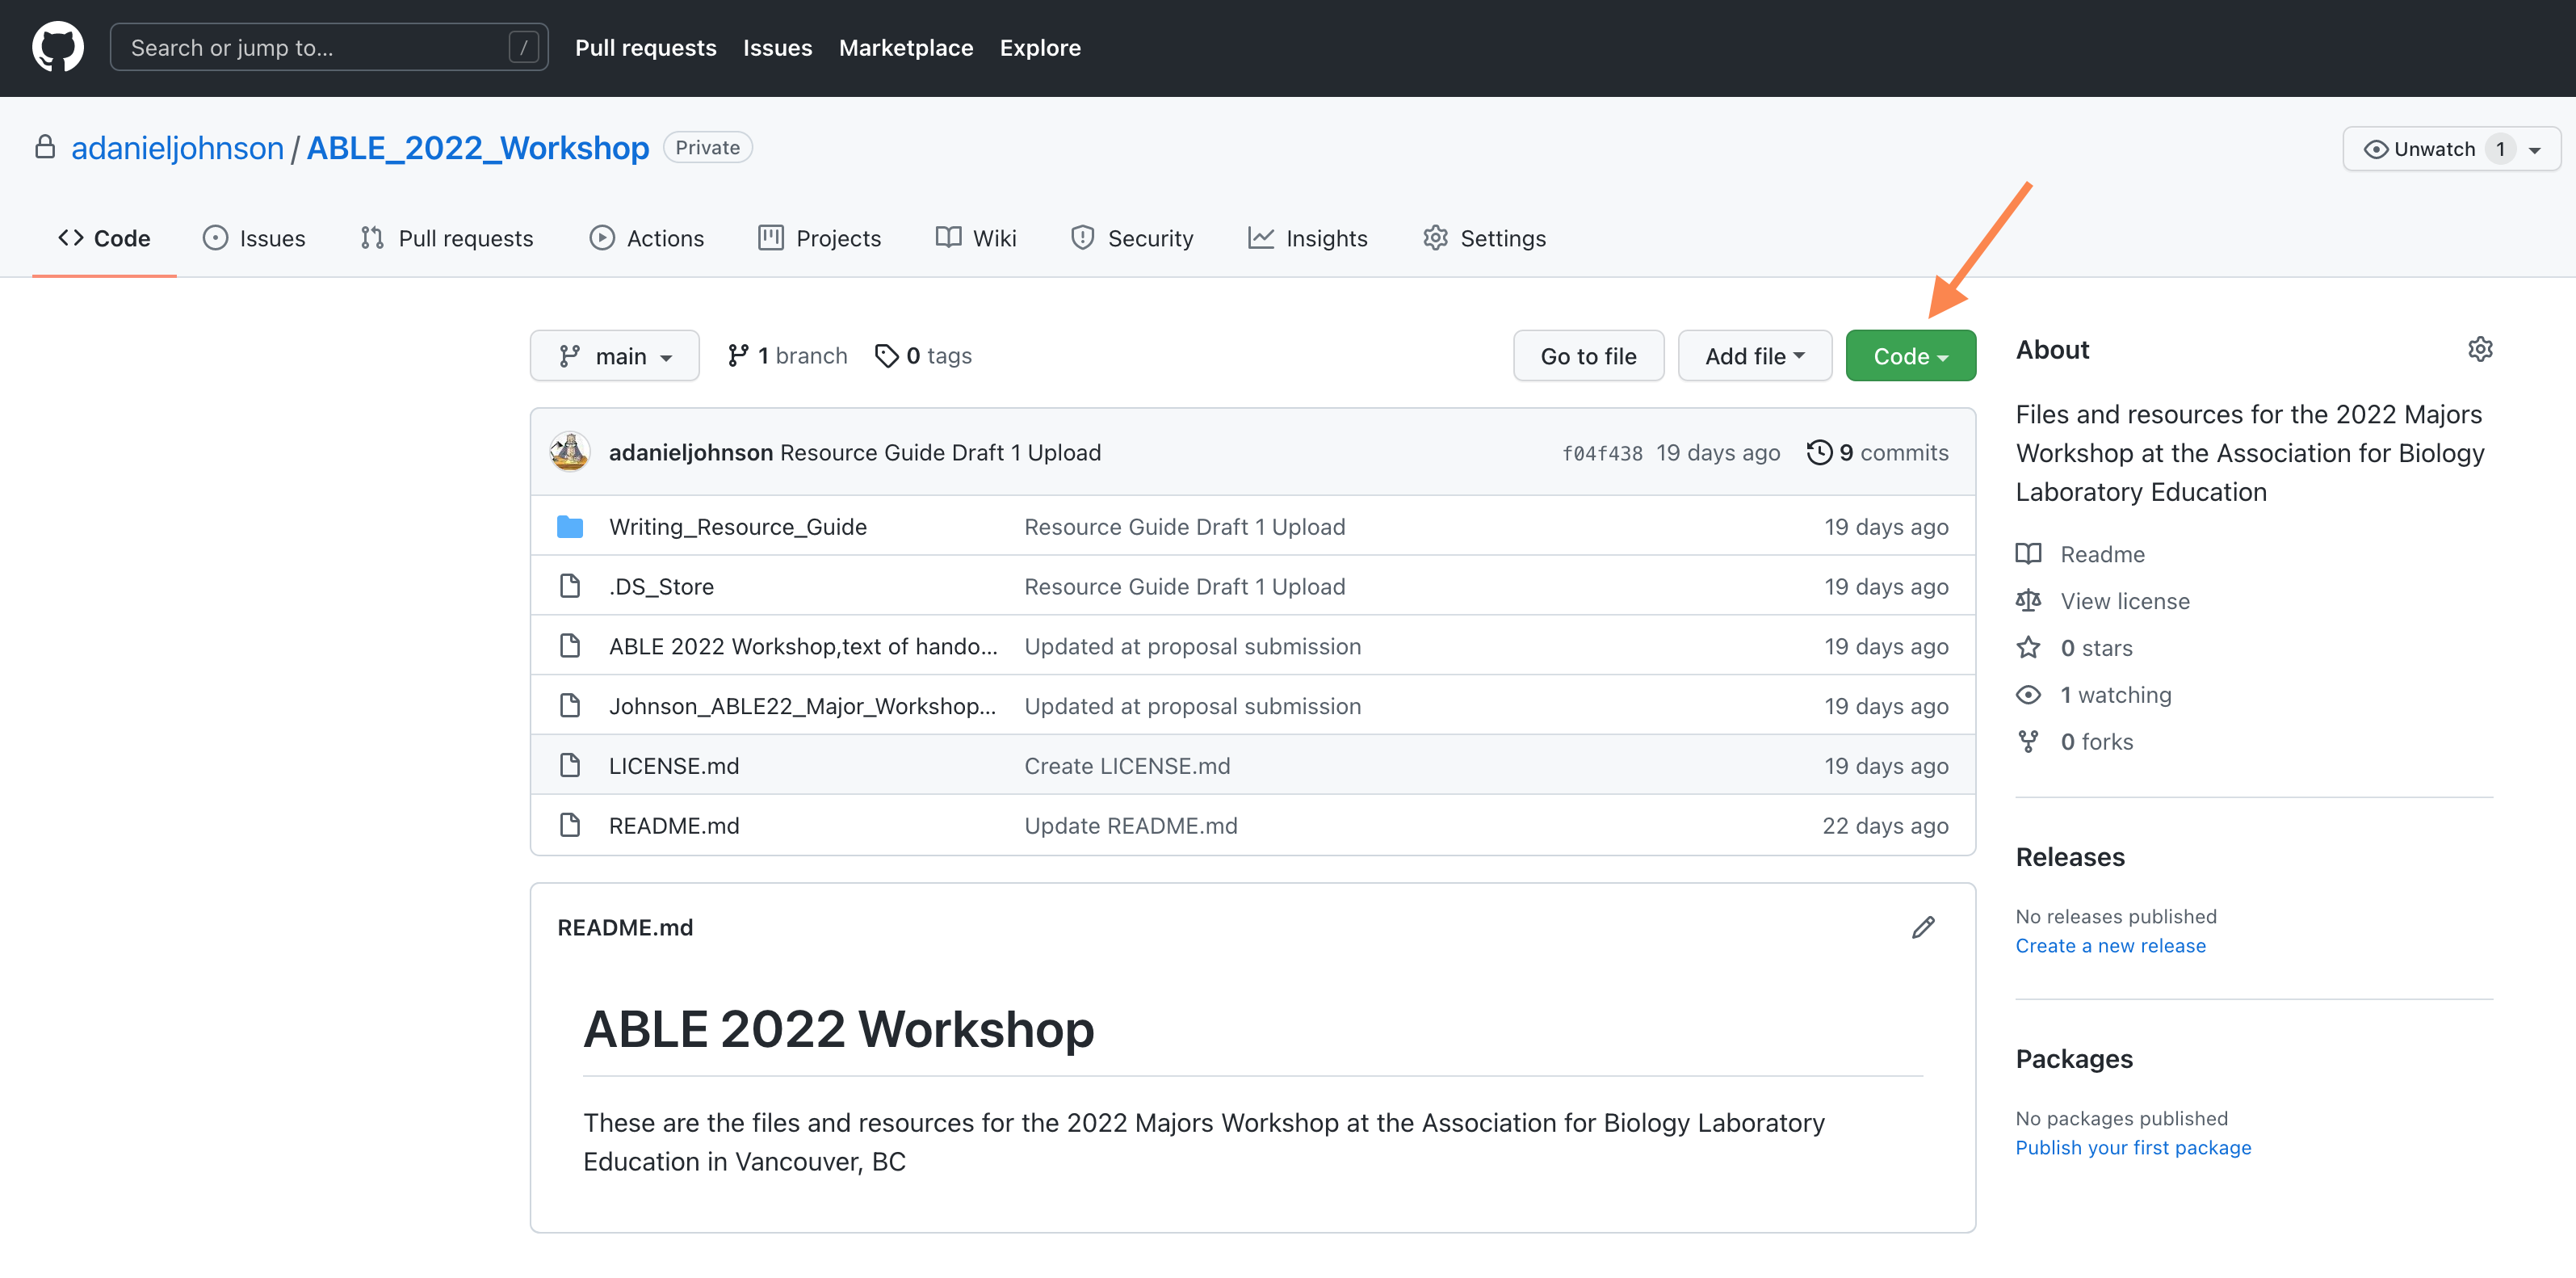
\includegraphics{https://github.com/adanieljohnson/ABLE_2022_Workshop/blob/main/images/Home-ABLE.png?raw=true}
\caption{Main page of ABLE Workshop repository}
\end{figure}

3. Click on ``Download ZIP'' (the BLUE arrow)

\begin{figure}
\centering
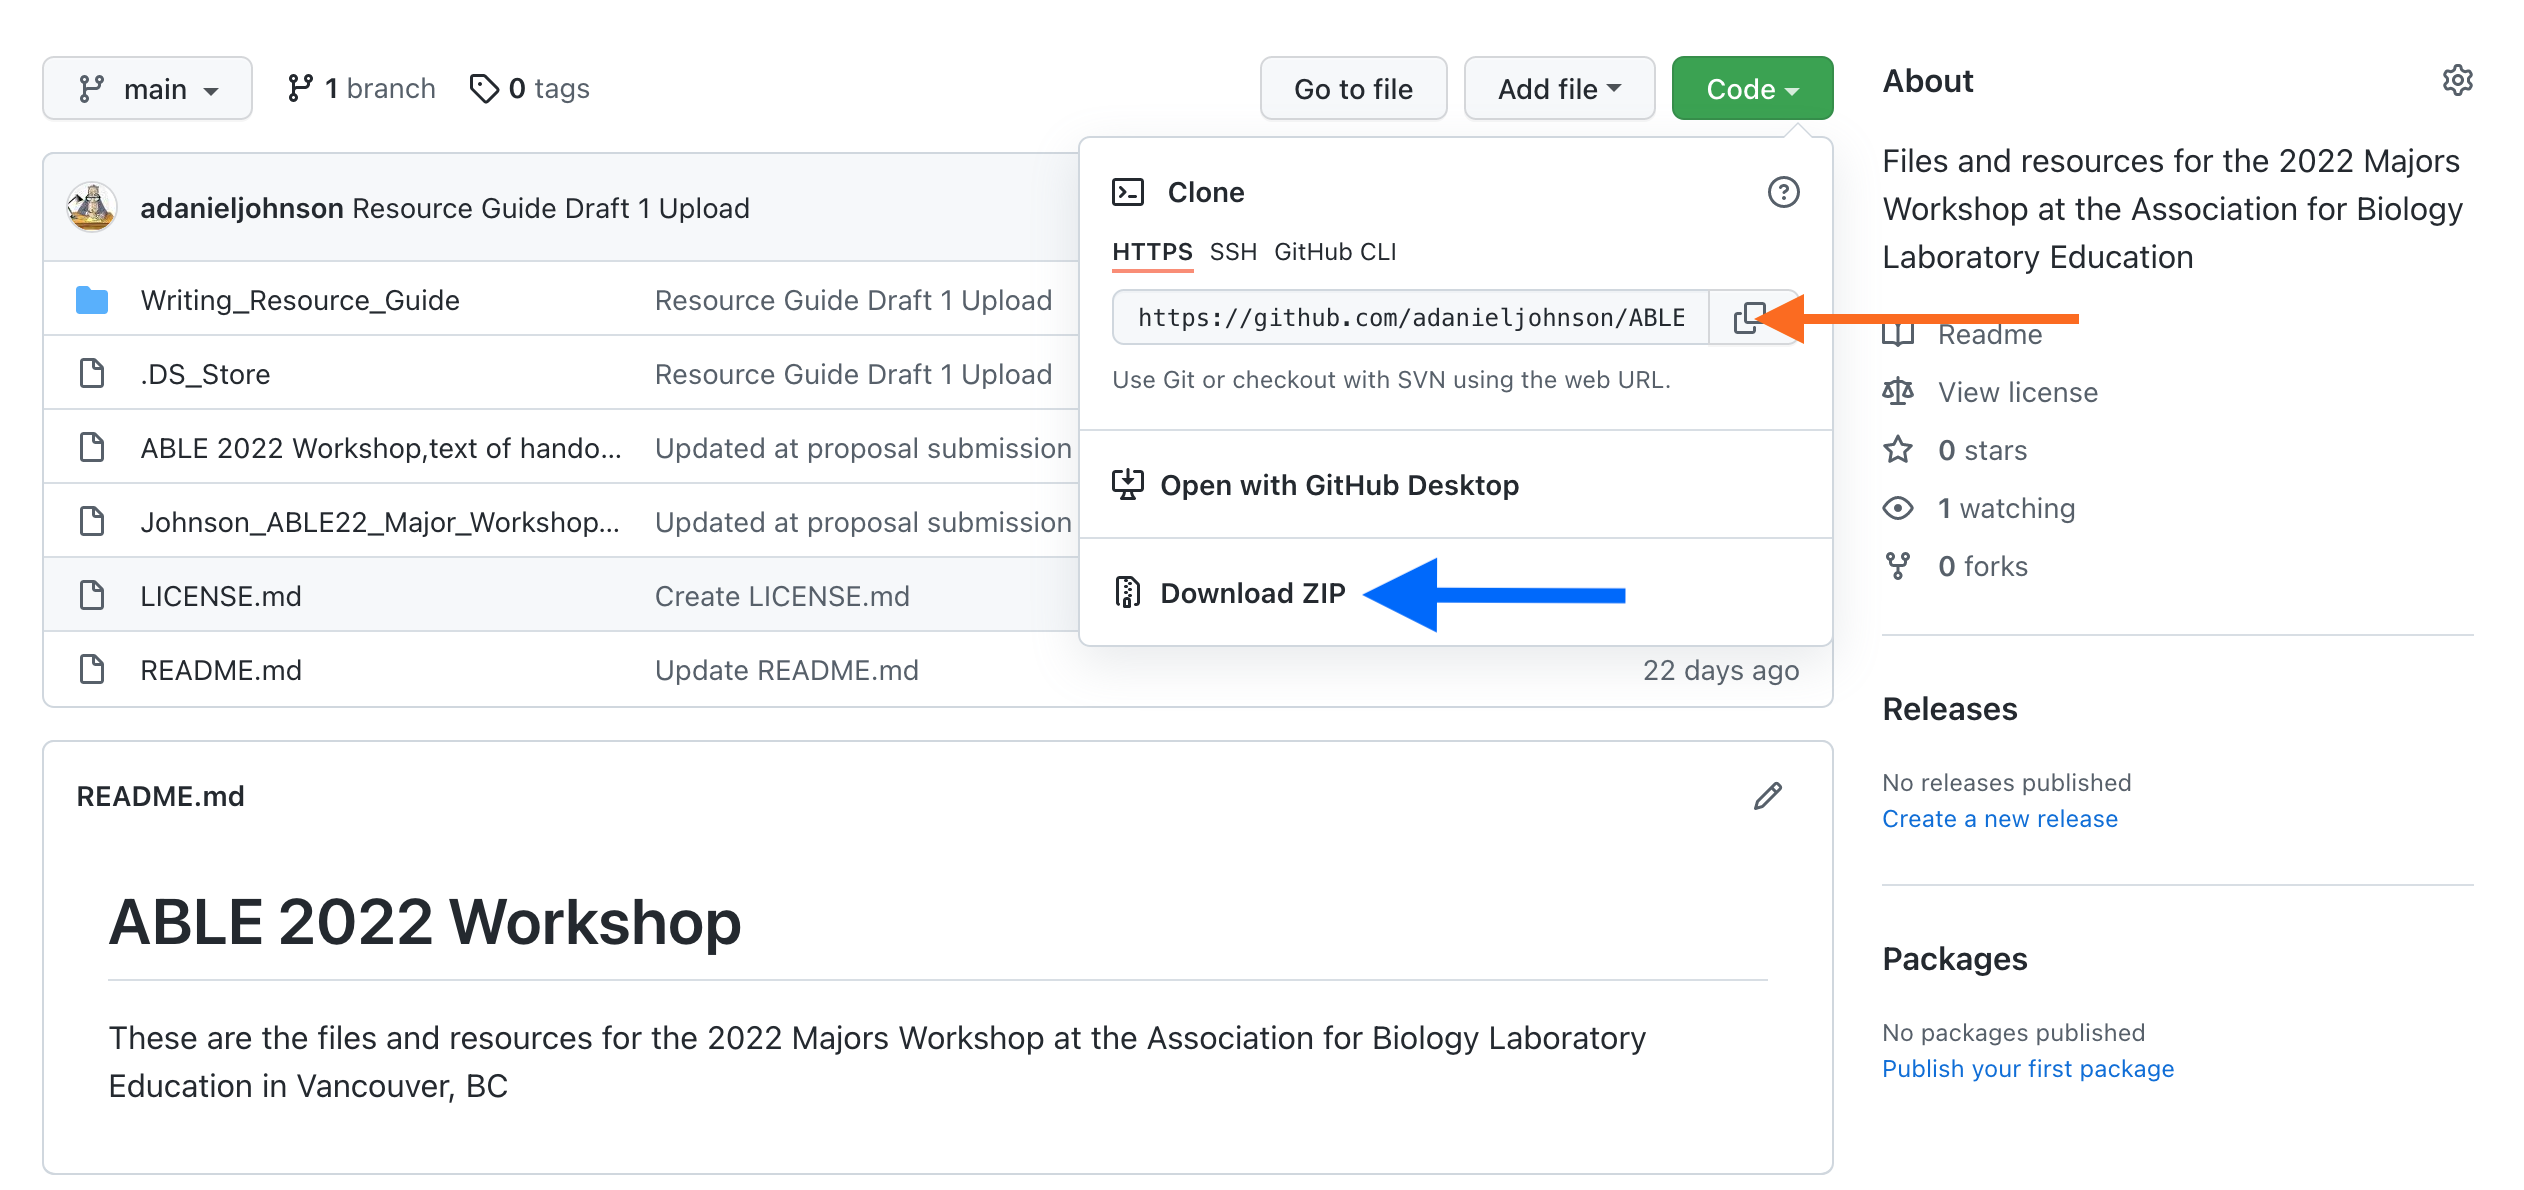
\includegraphics{https://github.com/adanieljohnson/ABLE_2022_Workshop/blob/main/images/Code-ABLE2.png?raw=true}
\caption{Blue arrow marks where to download a ZIP file.}
\end{figure}

4. The entire repo is over 70MB, so takes a minute to download. When it
is done, go to your Downloads folder and click to unpack the file.

5. Drag the unpacked folder to your desktop. Now you have a personal
copy of the files to work with. Do not worry about damaging any files.
If you need to replace a corrupted file, you can go back to the original
ZIP archive and unpack it again.

6. Open the folder named \textbf{Sample Files}. It contains .md files
and corresponding rendered HTML and MS Word files. Open ``ABLE
2022-Workshop\_1\_Source\_document.md'', then open either the
corresponding .html or .docx file.

7. Open \textbf{Handout for Exercise 1}; it will be your ``.md to
.html/.docx dictionary.'' Try to translate the markup in the .md files.
As you work, think about these questions:

\begin{itemize}
\tightlist
\item
  How hard or easy is it to read the \textbf{original text} in the .md
  file?
\item
  How does the markup translate into a web page?
\item
  How does the markup translate into a Word document?
\end{itemize}

8. If you make changes to your .md files, be sure to save them before
going on to Exercise 2.

\hypertarget{handout-for-exercise-1-short-guide-to-markdown}{%
\section{Handout for Exercise 1: Short Guide to
Markdown}\label{handout-for-exercise-1-short-guide-to-markdown}}

Markdown was created as a way for writers to annotate text quickly to
show formatting without having to embed full HTML tags. The goal with
Markdown is to separate the content (words of the text) of a document
from the format (headers, paragraphs, bullets, etc.) from the. By using
one well-defined set of marking conventions (called the
\textbf{syntax}), we can use converters to read a marked-up text and
render it to many different formats. For example, the converter we will
be using can read Markdown and export it in over 55 text formats.

\hypertarget{what-does-markdown-syntax-look-like}{%
\subsection{What Does Markdown Syntax Look
Like?}\label{what-does-markdown-syntax-look-like}}

Here is some text that has been formatted using Markdown:

\begin{center}\rule{0.5\linewidth}{0.5pt}\end{center}

\hypertarget{level-4-header---formatting}{%
\paragraph{Level 4 Header -
Formatting}\label{level-4-header---formatting}}

There are two main kinds of text formatting:

\begin{itemize}
\tightlist
\item
  Inline formatting (\emph{italics}, subscripts like
  H\textsubscript{2}SO\textsubscript{4}, etc.)
\item
  Block- or paragraph-level formatting (headings, sub-headings, lists,
  etc.)
\end{itemize}

\begin{center}\rule{0.5\linewidth}{0.5pt}\end{center}

Here is the same text that has been formatted so you can see the markup:

\begin{verbatim}
#### Level 4 Header - Formatting

There are two main kinds of text formatting:

* Inline formatting (_italics_, subscripts like H~2~SO~4~, etc.)
* Block- or paragraph-level formatting (headings, sub-headings, etc.)
\end{verbatim}

The number of hash (\#) marks indicates the level of the header. Lines
of text are separated by an extra space. Words or blocks of text that
have specific formatting are surrounded by a pair of symbols indicating
the type of formatting to apply. Here is what the same text looks like
rendered:

The rest of this handout explains the markup codes that you need most
often. Keep a copy handy until you can remember the specific codes
reliably. Better yet, copy the text of the original .md file and edit it
to suit your own needs.

\hypertarget{markdown-codes-for-inline-formatting}{%
\subsection{Markdown Codes for Inline
Formatting}\label{markdown-codes-for-inline-formatting}}

The table shows how to mark text, and what it will look like when
rendered.

\begin{longtable}[]{@{}
  >{\raggedright\arraybackslash}p{(\columnwidth - 4\tabcolsep) * \real{0.3333}}
  >{\raggedright\arraybackslash}p{(\columnwidth - 4\tabcolsep) * \real{0.3333}}
  >{\raggedright\arraybackslash}p{(\columnwidth - 4\tabcolsep) * \real{0.3333}}@{}}
\toprule
\begin{minipage}[b]{\linewidth}\raggedright
Inline Formats
\end{minipage} & \begin{minipage}[b]{\linewidth}\raggedright
How to Mark Them
\end{minipage} & \begin{minipage}[b]{\linewidth}\raggedright
How They Appear
\end{minipage} \\
\midrule
\endhead
Italics & \_italicized\_ word & \emph{italicized} word \\
& *italicized* word & \emph{italicized} word \\
Bold & \_\_bolded\_\_ word & \textbf{bolded} word \\
& **bolded** word & \textbf{bolded} word \\
Bold Italics & \_\_\_marked\_\_\_ word & \textbf{\emph{marked}} word \\
& ***marked*** word & \textbf{\emph{marked}} word \\
Superscripts & Super\^{}script\^{}ed letters &
Super\textsuperscript{script}ed letters \\
Subscripts & Sub\textasciitilde script\textasciitilde{} letters &
Sub\textsubscript{script}ed letters \\
Horizontal rule & *** & Draws a line across page \texttt{\_\_\_\_\_} \\
Inline code (not rendered) & `code block` & \texttt{code\ block} \\
Escape a special character &
\texttt{\textbackslash{}*code\ block\textbackslash{}*} & *code block* \\
Links to web pages & \texttt{{[}text{]}(link)} &
\href{https://www.rstudio.com}{RStudio} \\
Links with URL & \texttt{{[}link{]}(link)} &
\url{https://www.rstudio.com} \\
Embed local images &
\texttt{!{[}Image\ description{]}(path/to/local\_image).} &
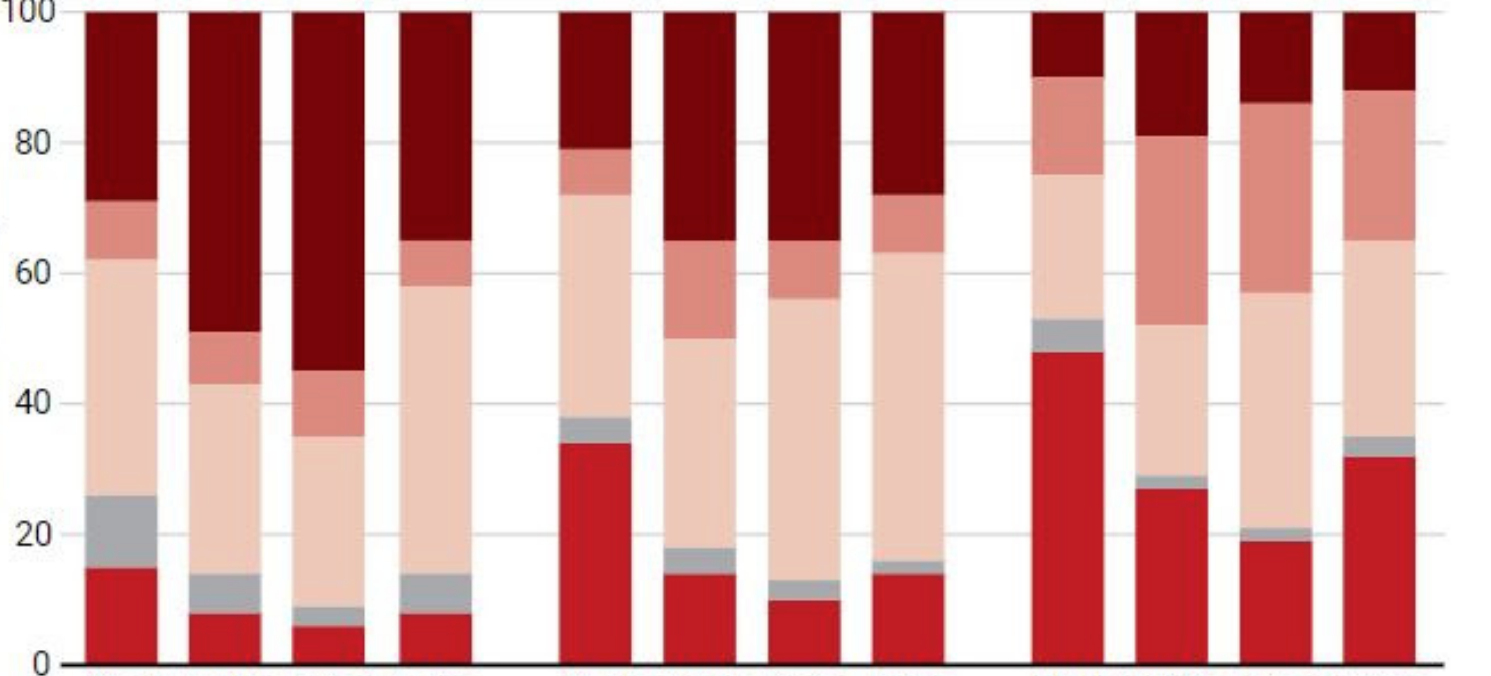
\includegraphics{https://github.com/adanieljohnson/ABLE_2022_Workshop/blob/main/images/desktop.png?raw=true} \\
Embed images from web &
\texttt{!{[}Image\ description{]}(URL\ for\ image).} &
\includegraphics{https://upload.wikimedia.org/wikipedia/commons/thumb/6/6c/Biology_students_in_lab.jpg/320px-Biology_students_in_lab.jpg} \\
\bottomrule
\end{longtable}

\hypertarget{codes-for-block-level-formatting}{%
\subsection{Codes for Block Level
Formatting}\label{codes-for-block-level-formatting}}

\hypertarget{headers}{%
\subsubsection{Headers}\label{headers}}

Header levels are indicated with 1-6 hash marks followed by a space.
These are the headers with the respective codes beneath each one.

\hypertarget{level-1-header}{%
\section{Level 1 Header}\label{level-1-header}}

\texttt{\#\ Level\ 1\ Header\ code} \#\# Level 2 Header
\texttt{\#\#\ Level\ 2\ Header\ code} \#\#\# Level 3 Header
\texttt{\#\#\#\ Level\ 3\ Header\ code} \#\#\#\# Level 4 Header
\texttt{\#\#\#\#\ Level\ 4\ Header\ code} \#\#\#\#\# Level 5 Header
\texttt{\#\#\#\#\#\ Level\ 5\ Header\ code} \#\#\#\#\# Level 6 Header
\texttt{\#\#\#\#\#\#\ Level\ 6\ Header\ code}

\hypertarget{paragraphs}{%
\subsubsection{Paragraphs}\label{paragraphs}}

Regular paragraphs need to be separated by a blank line, or they will
run together. For example, a text written like this, without spacing
lines:

\begin{verbatim}
    There are several kinds of text formatting to explore.
    Inline formatting text.
    Block- or paragraph-level formatting.
    Lists and quotes.
\end{verbatim}

Looks like this when rendered:

There are several kinds of text formatting to explore.Inline formatting
text.Block- or paragraph-level formatting.Lists and quotes.

Text written WITH spacing lines like this:

\begin{verbatim}
    There are several kinds of text formatting to explore.

    Inline formatting text.

    Block- or paragraph-level formatting.

    Lists and quotes.
\end{verbatim}

Renders like this:

There are several kinds of text formatting to explore.

Inline formatting text.

Block- or paragraph-level formatting.

Lists and quotes.

Blockquotes are written after the ``\textgreater{}'' symbol. A new
``\textgreater{}'' symbol is needed after each line break. This text:

\begin{verbatim}
> "I thoroughly disapprove of duels. If a man should challenge me,
  I would take him kindly and forgivingly by the hand and lead him
  to a quiet place and kill him."
>
> --- Mark Twain
\end{verbatim}

Renders like this:

\begin{quote}
``I thoroughly disapprove of duels. If a man should challenge me, I
would take him kindly and forgivingly by the hand and lead him to a
quiet place and kill him.''

--- Mark Twain
\end{quote}

\hypertarget{preventing-text-from-rendering}{%
\subsubsection{Preventing Text From
Rendering}\label{preventing-text-from-rendering}}

Blocks of text that should be displayed as written and not be rendered
are enclosed between three backticks. Blocks typed like this:

\texttt{\textasciigrave{}\textasciigrave{}\textasciigrave{}\ \ \ \ Block\ of\ text\ or\ code\ that\ should\ NOT\ be\ rendered,\ like\ this\ \_\_bold\_\_\ word.}
```

are rendered like this:

\begin{verbatim}
   Block of text or code that should NOT be rendered, like this __bold__ word.
\end{verbatim}

\hypertarget{hidden-comments}{%
\subsubsection{Hidden Comments}\label{hidden-comments}}

There are two ways to add comments to Markdown that will not display in
the rendered text:

\begin{verbatim}
[//]: # (This comment in Markdown gets removed from both .html, and .docx)

<!--- This comment in Markdown is retained in .html, gets removed from .docx-->
\end{verbatim}

\hypertarget{lists}{%
\subsection{Lists}\label{lists}}

Bulleted or unordered lists need to be separated from the preceding
paragraph by a blank line. The items start with *, +, or -, and you can
nest one list within another list by indenting the sub-list by four
spaces. For consistency, it is best to make it a habit of using one
character for main bullets, and the other two for sub-bullets.

A coded list looks like:

\begin{verbatim}
* First item
* Second item
    + First sub-item
        - First sub-sub-item
        - Second sub-sub-item
    + Second sub-item
* Third item
\end{verbatim}

The output renders as:

\begin{itemize}
\tightlist
\item
  First item
\item
  Second item

  \begin{itemize}
  \tightlist
  \item
    First sub-item

    \begin{itemize}
    \tightlist
    \item
      First sub-sub-item
    \item
      Second sub-sub-item
    \end{itemize}
  \item
    Second sub-item
  \end{itemize}
\item
  Third item
\end{itemize}

Ordered list items start with numbers, but the rule for nesting are the
same as for unordered lists.

\begin{verbatim}
1. First item
2. Second item
    1. First sub-item
        1. First sub-sub-item
        2. Second sub-sub-item
    2. Second sub-item
3. Third item
\end{verbatim}

The output renders as:

\begin{enumerate}
\def\labelenumi{\arabic{enumi}.}
\tightlist
\item
  First item
\item
  Second item

  \begin{enumerate}
  \def\labelenumii{\arabic{enumii}.}
  \tightlist
  \item
    First sub-item

    \begin{enumerate}
    \def\labelenumiii{\arabic{enumiii}.}
    \tightlist
    \item
      First sub-sub-item
    \item
      Second sub-sub-item
    \end{enumerate}
  \item
    Second sub-item
  \end{enumerate}
\item
  Third item
\end{enumerate}

The two formats can be mixed together:

\begin{verbatim}
1. First item
    + Sub-item
    + Sub-item
2. Second item
3. Third item
\end{verbatim}

Renders as:

\begin{enumerate}
\def\labelenumi{\arabic{enumi}.}
\tightlist
\item
  First item

  \begin{itemize}
  \tightlist
  \item
    Sub-item
  \item
    Sub-item
  \end{itemize}
\item
  Second item
\item
  Third item
\end{enumerate}

Numbered lists can be a bit fussy in Markdown. Sometimes they default to
starting with \#1. There is no simple and consistent way to force a list
to start with a particular number. I usually fix this by editing the
HTML or Word document directly, or just pre-number lists myself.

\hypertarget{math-expressions}{%
\subsection{Math Expressions}\label{math-expressions}}

Inline equations are written using standard LaTeX syntax, and enclosed
by pairs of \$ signs. This code:

\texttt{\$f(k)\ =\ \{n\ \textbackslash{}choose\ k\}\ p\^{}\{k\}\ (1-p)\^{}\{n-k\}\$}

Renders an inline version of the equation as:

\(f(k) = {n \choose k} p^{k} (1-p)^{n-k}\)

Equations in display style are written enclosed in a pair of double
dollar signs. This code:

\texttt{\$\$f(k)\ =\ \{n\ \textbackslash{}choose\ k\}\ p\^{}\{k\}\ (1-p)\^{}\{n-k\}\$\$}

Renders as:

\[f(k) = {n \choose k} p^{k} (1-p)^{n-k}\]

\textbf{Other Tips on Equations:}

\begin{itemize}
\tightlist
\item
  This link goes to a tutorial on
  \href{https://www.overleaf.com/learn/latex/Mathematical_expressions}{writing
  LaTeX equations}.
\item
  \href{https://latex.codecogs.com/legacy/eqneditor/editor.php}{Online
  equation builder} is a web page where you can write LaTeX equations
  using a visual editor.
\item
  Markdown equations sometimes fail to render correctly. Always check
  any formatted equations you have in a .md file the first time you try
  out a new rendering tool.
\item
  Unlike mathematicians, we usually do not need to edit equations after
  typing them the first time. So I usually will render them once, take a
  screen shot, and embed them as images. As with everything, whatever
  simplifies your workflow is what you should do, as long as you do it
  the same way every time.
\end{itemize}

\hypertarget{handy-html-bits}{%
\subsection{Handy HTML Bits}\label{handy-html-bits}}

There are some formats that Markdown does not handle well. For example,
subscript and superscript marks may not work on the first character or
number in a word (like 3H) or on a whole word. Some other useful items
are not in the GHFM syntax at all. You can fill in these gaps with a few
basic HTML codes.

\begin{longtable}[]{@{}
  >{\raggedright\arraybackslash}p{(\columnwidth - 4\tabcolsep) * \real{0.3333}}
  >{\centering\arraybackslash}p{(\columnwidth - 4\tabcolsep) * \real{0.3333}}
  >{\centering\arraybackslash}p{(\columnwidth - 4\tabcolsep) * \real{0.3333}}@{}}
\toprule
\begin{minipage}[b]{\linewidth}\raggedright
If you need to\ldots{}
\end{minipage} & \begin{minipage}[b]{\linewidth}\centering
Insert this HTML snippet
\end{minipage} & \begin{minipage}[b]{\linewidth}\centering
For this result
\end{minipage} \\
\midrule
\endhead
Force a superscript for a whole word or first character &
\texttt{\textless{}sup\textgreater{}super\textless{}/sup\textgreater{}script}
& superscript \\
Force a subscript for a whole word or first character &
\texttt{\textless{}sub\textgreater{}sub\textless{}/sub\textgreater{}script}
& subscript \\
Strike through text &
\texttt{\textless{}strike\textgreater{}This\textless{}/strike\textgreater{}\ word}
& This word \\
Add an extra space between items & \texttt{\&nbsp;} & \\
Add an extra line between items & \texttt{\textless{}br\textgreater{}}
& \\
Add a horizontal rule between lines &
\texttt{\textless{}hr/\textgreater{}} & \texttt{\_\_\_\_\_} \\
Add Greek letters & \texttt{\&alpha;,\ \&eta;} & α, η \\
\bottomrule
\end{longtable}

This page is a
\href{https://www.w3schools.com/html/html_formatting.asp}{good source
for other HTML shortcuts}. You can find more
\href{https://www.w3schools.com/html/html_symbols.asp}{information about
special symbols here}.

\hypertarget{learning-more}{%
\subsection{Learning More}\label{learning-more}}

These web resources can help you expand your Markdown writing skills.
More are listed in the Notes for Instructors.

\begin{itemize}
\tightlist
\item
  \href{https://docs.github.com/en/github/writing-on-github/getting-started-with-writing-and-formatting-on-github/basic-writing-and-formatting-syntax}{GitHub's
  Introduction to GHFM}
\item
  \href{https://www.pluralsight.com/guides/working-tables-github-markdown}{Making
  Tables in Markdown}
\item
  \href{https://www.tablesgenerator.com/markdown_tables}{Web-based
  Markdown Table Maker}
\item
  The \href{https://github.github.com/gfm/}{Official Specification for
  GHFM}. A \textbf{very} deep dive, but sometimes it is the best place
  to find answers to difficult formatting problems.
\end{itemize}

\hypertarget{exercise-2-creating-and-editing-markdown-pages}{%
\section{Exercise 2: Creating and Editing Markdown
Pages}\label{exercise-2-creating-and-editing-markdown-pages}}

\hypertarget{background-1}{%
\subsection{Background}\label{background-1}}

\hypertarget{why-use-markdown-instead-of-ms-word-or-google-docs}{%
\subsubsection{Why Use Markdown Instead of MS Word or Google
Docs?}\label{why-use-markdown-instead-of-ms-word-or-google-docs}}

Markdown is intended for the \textbf{start} of the authoring workflow.
\textbf{It assumes that text needs to be reused across multiple
formats.} MS Word is designed to produce polished print documents at the
end of the authoring and publication workflow. To that end, Word files
include a lot of hidden styling information that \textbf{limits
reusability.}

For example, if you have ever converted a long Word document into a web
page, or combined several documents into one, you probably have seen
unpredictable changes in format. This happens because of the embedded,
hidden styling information. Markdown does not hide the formatting
information, making it much easier to combine and convert documents.

What other advantages does Markdown have beyond ``write once, reuse many
ways''?

1. Markdown files are \textbf{VERY} small compared to Word .docx files.
For example, the Markdown file containing the full set of handouts for
this workshop is 54KB; the corresponding Word file is 3.8 MB (70x
larger.)

2. Markdown files do not have embedded images. They use an address to
``call in'' images when the document is rendered. One master set of
images can be stored in a single location and called into any Markdown
document. If an image is updated, every document or web site that uses
that image will use the new version the next time the file is generated.

3. When a Markdown file is converted to another format, all of the
headers, bold words, etc., get tagged with appropriate styling codes for
that document type. This greatly reduces time spent reformatting
converted documents.

\begin{itemize}
\tightlist
\item
  Say you create a long document, convert it to Word, and decide you
  want to change all 155 section headers from blue to red text in a
  different font. You do not have to convert each header one at a time;
  change the master style settings for headers once, and every header
  changes.
\item
  If you copy/paste Markdown HTML into an existing site (like an LMS
  page), the added text adopts the styles of its new location.
\end{itemize}

4. Markdown is truly platform-agnostic. The same file can be edited on a
Mac, a PC, and a Linux machine, and never have any compatibility
problems.

5. Markdown and the tools needed to convert it are available for free.

\hypertarget{how-do-we-create-markdown-documents}{%
\subsubsection{How Do We Create Markdown
Documents?}\label{how-do-we-create-markdown-documents}}

Markdown files are plain text files with \textbf{.md} as the extension.
Unlike HTML, Markdown does not require any additional special code or
starting text at the beginning of a new document. The file extension is
the only requirement.

There are many ways to write Markdown files. You can:

\begin{itemize}
\tightlist
\item
  Use a plain text editor on your computer. If you need to share your
  documents in many different places or formats, or are not sure where
  they will go, writing them in a standalone text editor is probably
  easiest.
\item
  Write them entirely inside R Studio. R Studio includes a fairly good
  plain text editor. If you plan to manage your files entirely through R
  Studio, it makes sense to write your text files there too.
\item
  Write text files inside GitHub via a browser. If you want to be 100\%
  sure you never lose a single word, and don't mind a few extra steps,
  writing directy in GitHub might be best. Files written in GitHub via a
  browser are saved immediately to their repository: no pulling or
  pushing needed. If you use R Studio or a standalone editor you will
  have to commit and push changes to GitHub from time to time.
\end{itemize}

Which will work best for you depends on your personal preferences, and
how you plan to use the files. You may end up using some of all three
methods. The goal of this exercise is to introduce you to each method,
so you can find a workflow that feels comfortable to you.

\begin{quote}
\textbf{Personal Tidbit:} my own workflow changes with what I am doing.
Right now, most of my writing ends up on our campus LMS so it needs to
be plain HTML. Occasionally I write handouts that need to be in MS Word
(.docx) format. I prefer to write drafts in a commercial plain text
editor that shows Markdown codes in color. I work across multiple
computers, so even my early draft files go into a GitHub repository so I
can access them anywhere.

When it is time to generate output, the text editor I use converts
Markdown directly to plain HTML that I can copy/paste straight into our
LMS. I use R Studio to generate MS Word documents and build online
books. I rarely make PDFs anymore because they are hard for screen
readers to translate.
\end{quote}

In this exercise you will try writing and editing Markdown texts using R
Studio as a text editor, then using a standalone text editor. Your goal
is to experience for yourself how Markdown behaves in different editing
environments. One probably will feel more comfortable than the other;
that is the way you should start out building your editing workflow.

\hypertarget{procedure-1}{%
\subsection{Procedure}\label{procedure-1}}

\hypertarget{editing-markdown-using-r-studio}{%
\subsubsection{Editing Markdown Using R
Studio}\label{editing-markdown-using-r-studio}}

1. Open R Studio, choose \textbf{File \textgreater{} Open} and navigate
to your copy of the \textbf{ABLE 2022 Workshop} repository. Open to the
file containing the \textbf{Table of Contents} page for the Writing
Resource Guide.

2. Find 1-2 EXISTING pages you think you might want to edit or
contribute to. Also find 1-2 topics that you do not see in the current
pages that you think should be in the Guide.

3. Now open the folder named \textbf{Writing Resource Guide.} It
contains the Markdown files (with the ``.md'' extension) for the full
Writing Resource Guide. Locate one of the pre-existing .md files you
wanted to edit, and open it.

\begin{itemize}
\tightlist
\item
  First look at the current structure. If needed, compare it to the
  markup guide in the handout from earlier. Do you see how the structure
  of the rendered file is encoded in the Markdown tags? (If needed, you
  can click the \textbf{Preview} tab at the top of the window to switch
  from Code to Preview modes.)
\item
  Look for a section you want to edit. Make some changes, save, then see
  how your changes look using \textbf{Preview} mode.
\end{itemize}

4. Next you will start a new file. Choose \textbf{File \textgreater{}
New File \textgreater{} Markdown file} (orange arrow). Do NOT use R
Markdown (the blue arrow).

\begin{figure}
\centering
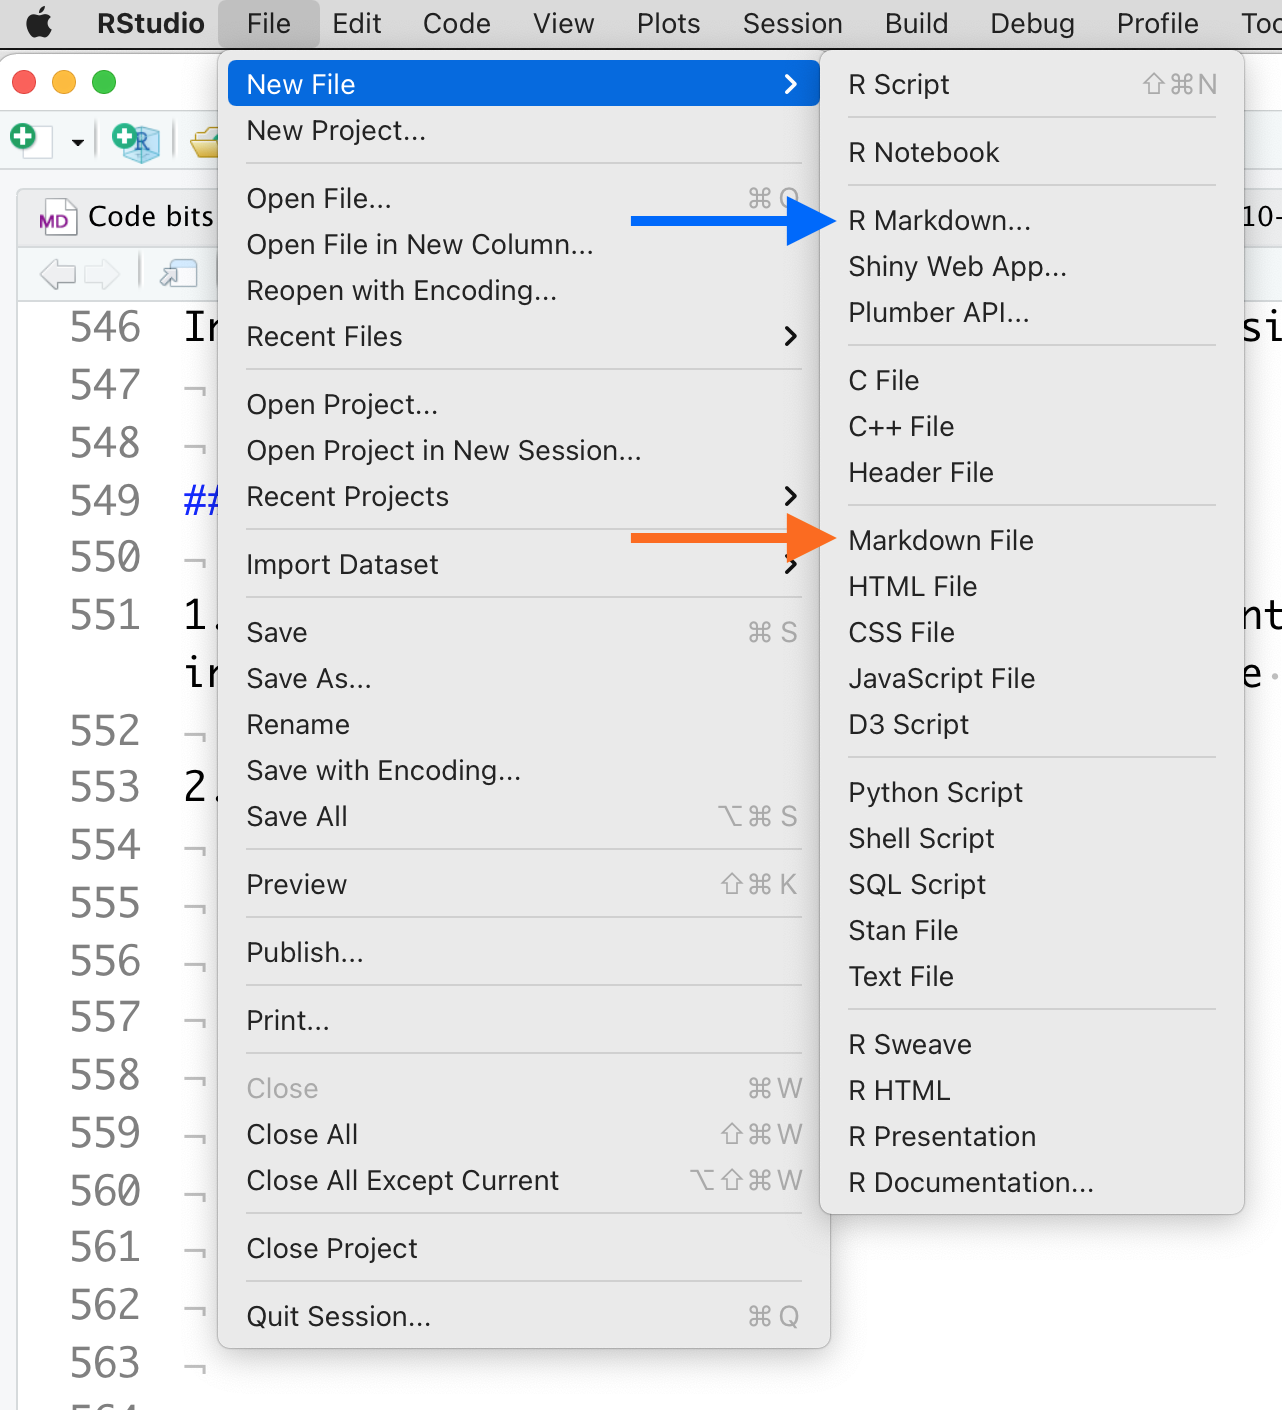
\includegraphics{https://github.com/adanieljohnson/ABLE_2022_Workshop/blob/main/images/Start-MD-ABLE.png?raw=true}
\caption{Start a new .md file}
\end{figure}

5. Enter some starting text. One or two words is enough.

6. Save the file in your \textbf{ABLE 2022 Workshop} folder. Give your
file a name that reflects the topic you did not see. Include the .md
extension. \textbf{TIP:} do not include spaces in file names. Write all
file names in CamelCase (FileName1.md) or Snake\_Case (File\_Name\_1.md)

7. Now you have a starting file that you can edit any way you wish.

\begin{itemize}
\tightlist
\item
  If you want to see how changes to the Markdown code affect it, click
  the \textbf{Preview} button at the top of the window.
\item
  If the .md file will not display, you probably have an error in the
  format. Look at the bottom of the page for a tab called \textbf{R
  Markdown}. There usually is an error message telling you what went
  wrong.
\end{itemize}

8. When you are finished editing your 1-2 pages, save them both in the
\textbf{ABLE 2022 Workshop} folder.

9. Close R Studio for now.

\hypertarget{editing-markdown-using-a-plain-text-editor}{%
\subsubsection{Editing Markdown Using a Plain Text
Editor}\label{editing-markdown-using-a-plain-text-editor}}

1. Navigate to your \textbf{ABLE 2022 Workshop} folder on your desktop.

2. Click on one of the .md files in the \textbf{Writing Resource Guide}
folder to select it. This time you want to open the file in a plain text
editor.

\begin{itemize}
\tightlist
\item
  For Windows, the default text editor is
  \href{https://notepad-plus-plus.org/}{\textbf{Notepad++}}. If you do
  not have it, you can install it in \textasciitilde1 minute by clicking
  on the link above.
\item
  For MacOS, \textbf{TextEdit} is the default pre-installed editor.
\item
  You can open and edit .md files with any text editor you have
  installed, such as \href{https://brackets.io/}{Brackets},
  \href{https://bluefish.openoffice.nl/index.html}{Bluefish},
  \href{https://www.barebones.com/products/bbedit/}{BBEdit},
  \href{https://atom.io/}{Atom}, etc.
\item
  If you have no idea what text editor you have installed, just
  double-click the file. Your operating system will try to open the file
  with the appropriate program.
\end{itemize}

3. After you have edited an existing .md file, try creating a new one
from scratch. Once again, create a new file for a topic you think is
missing from the Table of Contents of the Resource Guide.

4. When you have finished, save both of your edited .md files.

\hypertarget{writing-tips-and-tricks}{%
\subsubsection{Writing Tips and Tricks}\label{writing-tips-and-tricks}}

\begin{itemize}
\tightlist
\item
  Always start Markdown pages with a Level 1 header that is the title of
  the document. Reserve the Level 1 header just for that purpose. This
  does not seem very useful at first, but it becomes essential when you
  start compiling multiple .md files into longer documents or books.
\item
  It is tempting to remove spaces between lines of text in .md files.
  BAD idea! Markdown relies on blank lines to keep track of blocks of
  text. When Markdown is rendered, extra blank lines are deleted
  automatically.
\end{itemize}

\hypertarget{common-novice-questions-and-mistakes}{%
\subsubsection{Common Novice Questions and
Mistakes}\label{common-novice-questions-and-mistakes}}

\begin{itemize}
\tightlist
\item
  We will build this list together during the workshop.
\end{itemize}

\hypertarget{exercise-3-generating-output-documents}{%
\section{Exercise 3: Generating Output
Documents}\label{exercise-3-generating-output-documents}}

\hypertarget{background-2}{%
\subsection{Background}\label{background-2}}

In Exercises 1-3 you learned how to create, edit, and manage Markdown
files. Now we are going to create documents with those files. There are
several Markdown file processors. We will be working with
\href{https://pandoc.org/index.html}{\textbf{Pandoc}}, a ``universal
document converter.'' It can read many different document file types,
then convert one format to another. Some file types get fussy when
converted, but Markdown and Pandoc play very nicely together.

There are several ways to access Pandoc; you do not need to work with it
directly. In this exercise you will:

\begin{itemize}
\tightlist
\item
  Use a web-based converter to create clean HTML, and
\item
  Use R Studio to create MS Word documents.
\end{itemize}

I will demonstrate two other routes:

\begin{itemize}
\tightlist
\item
  Using the command line to build single files, and
\item
  Using R Studio's bookdown package to compile single files into an
  e-book.
\end{itemize}

\hypertarget{procedure-converting-text.md-to-text.html}{%
\subsection{Procedure: Converting Text.md to
Text.html}\label{procedure-converting-text.md-to-text.html}}

Many plain text editors (though oddly, not R Studio) can convert
Markdown to very compact plain HTML. If your text editor does not have
this feature, this web-based Pandoc converter works well.

1. Go to the \textbf{MD to HTML Converter} at
\href{https://ashkanph.github.io/md-to-html/}{https://ashkanph.github.io/md-to-html/.}

2. In the upper right corner, use \textbf{Browse} to find your local
GitHub folder, and choose one of your recently edited .md files.

3. The .md file will be converted to .html and displayed.

4. Use the \textbf{Save as HTML} button to write a copy of the file in
.html back to your local GitHub folder.

5. If you open the version of the file with the .html extension in your
plain text editor, you will see it has been rewritten using HTML markup.
You can copy and paste the HTML code into most LMS pages. Alternatively,
you can share the file itself with others; they can open it in any web
browser.

\begin{quote}
\textbf{Why not use R Studio for HTML?} When R Studio generates
standalone HTML files, it embeds the raw code for every image plus a LOT
of extra styling code. For example, the HTML file containing the
handouts for this workshop that was generated using the Ashkanph
converter is 63 Kb. The same HTML file generated using R Studio is 6 Mb.
This problem goes away when R Studio creates books; the HTML files are
very compact, because they reference separate styling and image files
rather than embedding them.
\end{quote}

\hypertarget{other-options-for-html}{%
\subsubsection{Other Options for HTML}\label{other-options-for-html}}

There are many free MD to HTML converters available. Two very good ones
are \textbf{\href{https://markdown-it.github.io/}{Markdown It}} and
\textbf{\href{https://markdowntohtml.com/}{Markdown to HTML}}; both have
very user-friendly interfaces, but require copy/pasting the text rather
than choosing a file.

\textbf{\href{https://dillinger.io/}{Dillinger}} is a web-based editor
that shows the Markdown code in a window next to either the HTML code or
the styled text. Rendered Markdown can be exported as HTML, but like R
Studio, Dillinger includes some extra styling information.

If you prefer to use a standalone Markdown editor,
\textbf{\href{http://pad.haroopress.com/}{HarooPad}} produces both clean
and styled forms of HTML. HarooPad has some trouble with equations.

\hypertarget{procedure-converting-text.md-to-text.docx}{%
\subsection{Procedure: Converting Text.md to
Text.docx}\label{procedure-converting-text.md-to-text.docx}}

R Studio is very good for converting .md files to well-formatted Word
documents.

1. Open R Studio, and go to the workshop files. Open one of the files
you edited or created.

2. At the top of the screen, open the pulldown menu next to
\textbf{Preview} and choose \textbf{Word document}.

\begin{figure}
\centering
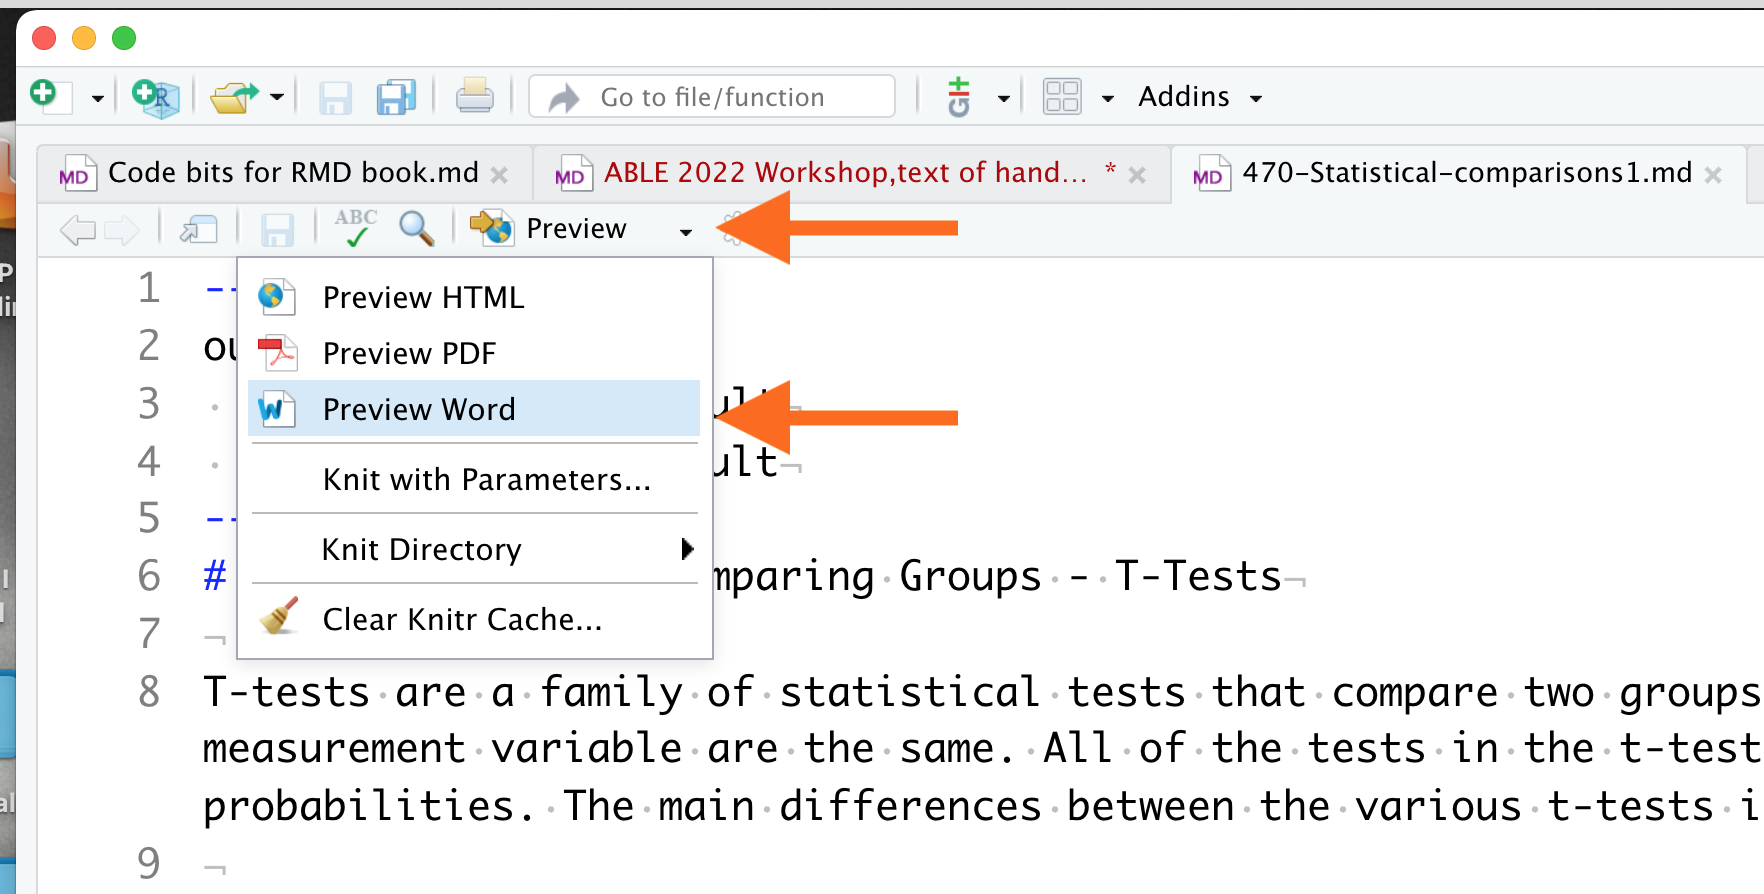
\includegraphics{https://github.com/adanieljohnson/ABLE_2022_Workshop/blob/main/images/Preview-Word-ABLE.png?raw=true}
\caption{Converting Markdown to Word format}
\end{figure}

3. R Studio will call Pandoc, generate a pre-formatted MS Word .docx
file, then save it to the same directory where the .md file is located.

4. Click on the .docx file to open it in MS Word.

MS Word files are formatted using a standard template. To reformat
documents a different way, create a template file with the header and
text styles that you want. When newly generated documents are
copy/pasted into the template file, the text will change to the styles
you set.

\hypertarget{demonstration-1-running-pandoc-from-the-command-line}{%
\subsection{Demonstration 1: Running Pandoc From the Command
Line}\label{demonstration-1-running-pandoc-from-the-command-line}}

It is very easy to install and run Pandoc from your computer's command
line, and it generates both .docx and .html files. If you would like to
follow along and try it yourself:

1. Go to the \href{https://pandoc.org/installing.html}{Pandoc
installation page} for instructions to download and install to your
computer.

2. Use the following Terminal commands to convert from .md to .html or
.docx format. The commands are the same, except for the extension on the
output file.

\begin{verbatim}
    pandoc -s /filepath/Input_Filename.md  -o /filepath/Output_Filename.html

    pandoc -s /filepath/Input_Filename.md  -o /filepath/Output_Filename.docx
\end{verbatim}

Pandoc is fussier about rendering PDFs. First, it does not tolerate
markup errors, and may refuse to convert a file. Second, you must
install a pdf-engine then call it in the command. Look at the example
below:

\texttt{pandoc\ -s\ -\/-pdf-engine=xelatex\ /filepath/Input\_Filename.md\ \ -o\ /filepath/Output\_Filename.pdf}

The pdf-engine defines what the format will look like. This particular
PDF engine's default layout and fonts look outdated and can be hard to
read. Changing them requires some deeper coding work, which is why I do
not recommend using Pandoc for creating occasional PDFs. It is quicker
to render a file in MS Word then save it as a PDF.

You are not limited to PDF, HTML, and DOCX files. Pandoc can convert
Markdown files into slides, bibliographic formats, Jupyter notebooks,
CSV data files, and multiple wiki languages too.
\href{https://pandoc.org/}{This list} shows all of the possible
conversions you can do.

\hypertarget{demonstration-2-using-rs-bookdown-to-compile-documents}{%
\subsection{Demonstration 2: Using R's Bookdown to Compile
Documents}\label{demonstration-2-using-rs-bookdown-to-compile-documents}}

R has powerful libraries for creating online materials. The
\textbf{bookdown} package (which uses \textbf{knitr} plus Pandoc)
combines individual .md files into full length technical books. The
\textbf{\href{https://bookdown.org/}{Home page for the R Bookdown
package}} has examples of books that were created this way.

There is not enough time for you to set up your own GitHub-hosted book
from start to finish. Instead, we'll take a short tour through the back
end of the \textbf{SWP Writing Resource Guide} and see how R Studio can
turn a collection of separate .md files into an integrated book.

We also will talk about what is \textbf{missing} from the Resource Guide
that you added, and your suggestions for improving it.

\hypertarget{exercise-4-using-github-to-back-up-manage-and-write-files}{%
\section{Exercise 4: Using GitHub to Back Up, Manage, and Write
Files}\label{exercise-4-using-github-to-back-up-manage-and-write-files}}

\hypertarget{background-3}{%
\subsection{Background}\label{background-3}}

Up to now you have edited and saved your .md files locally. Now we are
going to create a local repository on your computer and clone it to your
GitHub account. This serves both as a backup copy of your work AND a way
to share it with others.

\begin{quote}
\textbf{Do I HAVE to use GitHub?} Nope, it is entirely up to you. You
can copy files from any GitHub public repository; only the private
repositories are restricted to account holders. If you never share files
with other people, only work with local copies, and have a good back-up
service already, then you may not need it.

GitHub has many benefits though. You can share files with others, get
their suggestions, then decide whether or not to incorporate them. If
you work across multiple computers (home and work for example), GitHub
helps ensure you always are working on the most recently updated files.
You also can set up a personal web site for each repository you have. If
you are interested in using R or data science tools in your lab courses,
then you definitely want to become comfortable using GitHub.
\end{quote}

GitHub has two functions that help you keep repositories in sync:
\textbf{pull} (sometimes called \textbf{fetch}) and \textbf{push}. These
commands can be confusing, but they are at the heart of what makes
GitHub so powerful.

When you pull (or, fetch) a copy of a repository, GitHub compares the
versions of the files in the repository on its servers and your local
computer. If the server version does not match the local version
exactly, GitHub will try to download the newer version and update the
older version on your local computer. If there are newer versions in
BOTH locations, GitHub will ask you to pick one to be the new
``correct'' version.

Say you have been editing several .md files using the text editor on
your computer. When you \textbf{commit} the files, you are telling
GitHub ``these are the newest versions, and what everyone should be
using from now on.'' GitHub dutifully stamps them with a time and
location code, and stores them locally. You need to \textbf{push} the
files to tell the main GitHub server to update its copies.

When you push files, the server compare its copy of each file to the
data stamp on the one you pushed. If there are changes in the server
copy that are not in yours, GitHub will stop and tell you that you need
to pull the changes already logged by the server and merge them with
your local changes first. \textbf{Then} you can push the newest version
of each file back to the server. This is a quirk of GitHub; usually
pulling from the server resolves any conflicts.

\begin{quote}
\textbf{Why does GitHub use so many different commands?} Why not just
save a file instantly and everywhere, like Google does? If you have ever
had someone change a Google document you just finished editing back to
what you deleted, you know why. GitHub's strategy is designed for code
writers and editors. There has to be one ``correct'''' version, and one
person with the authority to make the decision what files are correct.
Committing a file only saves it to the local copy of the repository you
happen to be working in. Pushing a file changes it on the main server,
and on all of the forked copies.
\end{quote}

\hypertarget{procedure-2}{%
\subsection{Procedure}\label{procedure-2}}

1. Open GitHub . If you are not logged in to your account, do so now. If
you did not sign up for GitHub, partner with someone who did and watch
the process.

2. At the top right is a button to access your account. Click on
\textbf{My Repositories.}

\begin{figure}
\centering
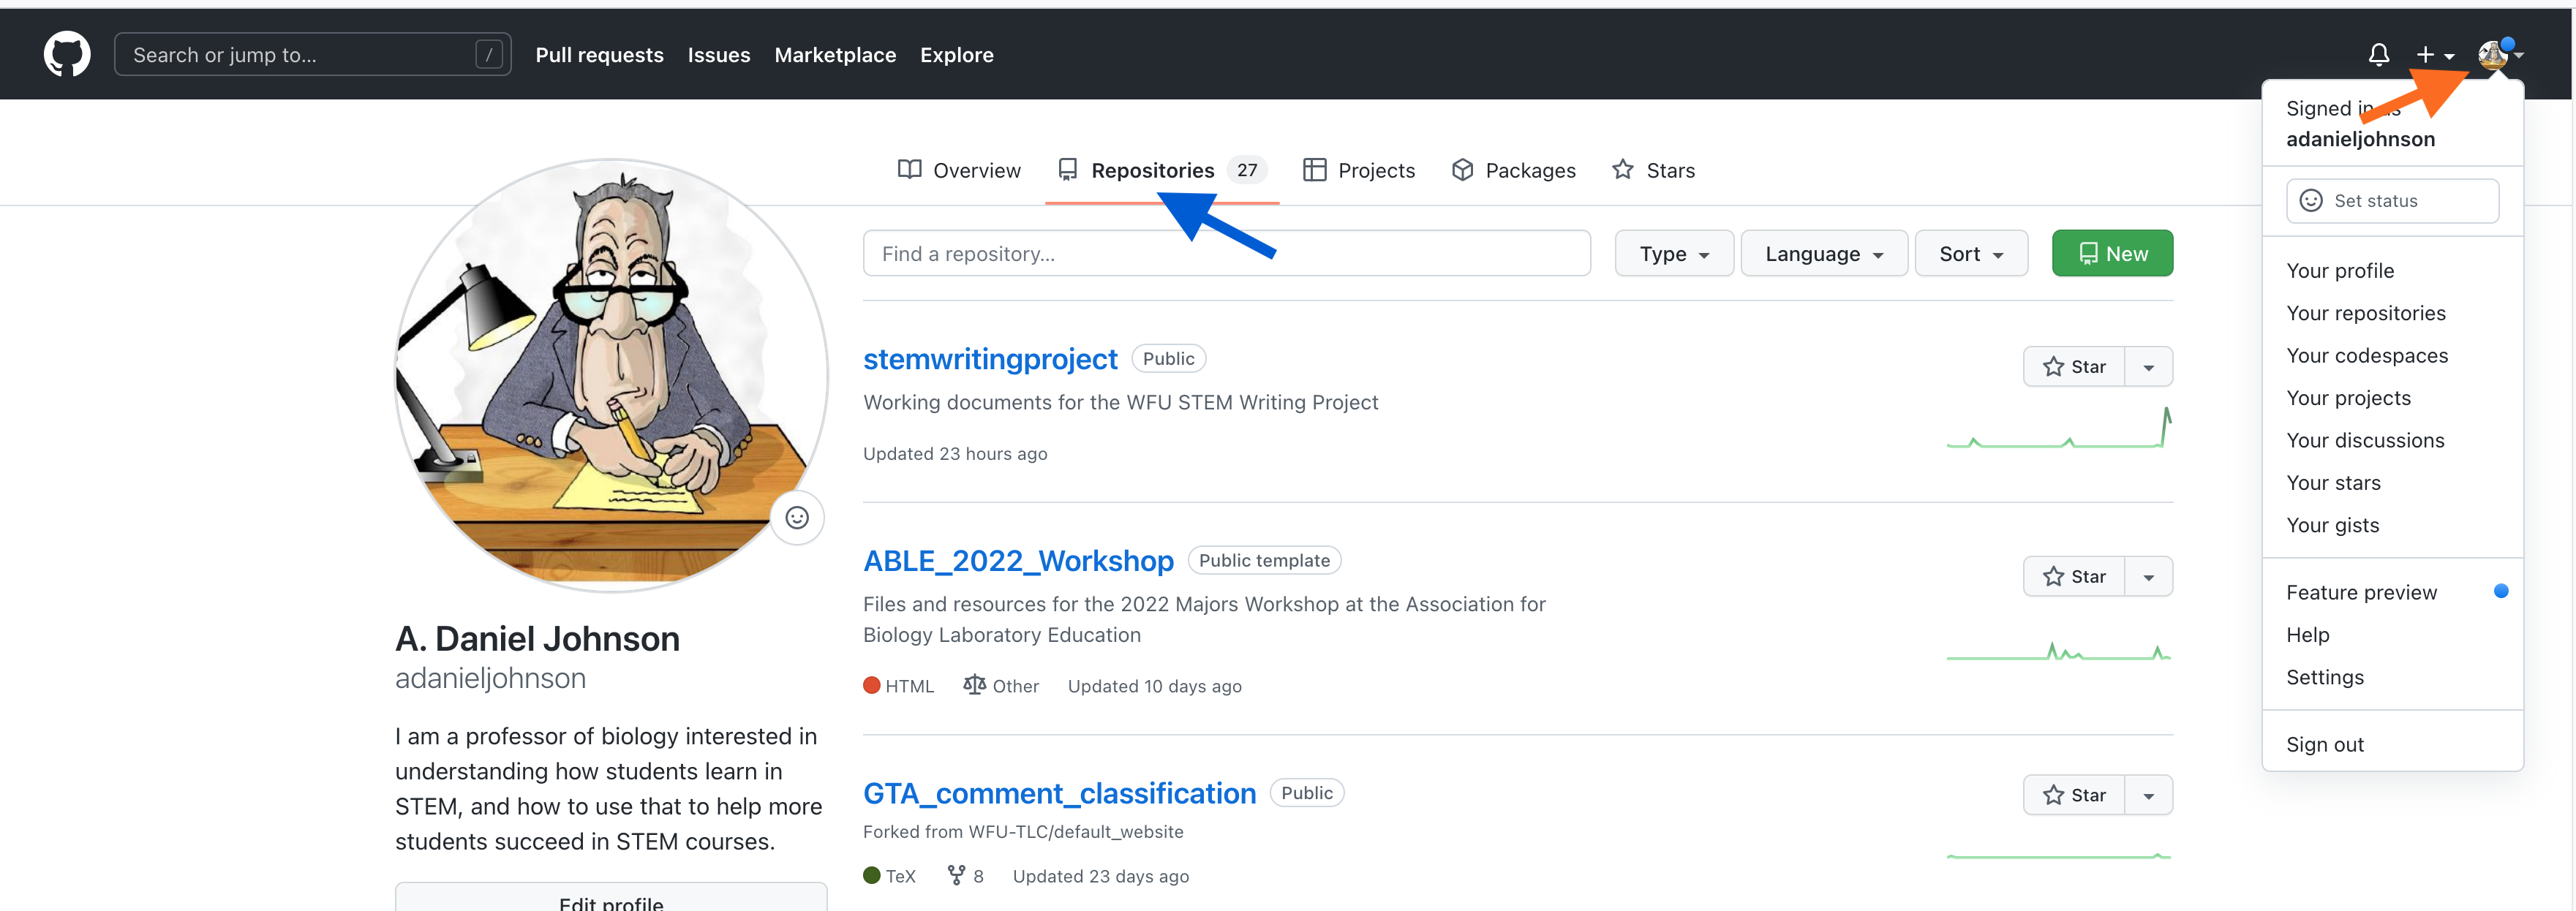
\includegraphics{https://github.com/adanieljohnson/ABLE_2022_Workshop/blob/main/images/Access_account.png?raw=true}
\caption{Accessing your account (orange arrow) and your repositories
(blue arrow).}
\end{figure}

3. You will not have any repositories yet. Click on New.

4. Give your repository a short name in CamelCase or Snake\_Case. Skip
the other items and click on \textbf{Create Repository}.

\begin{figure}
\centering
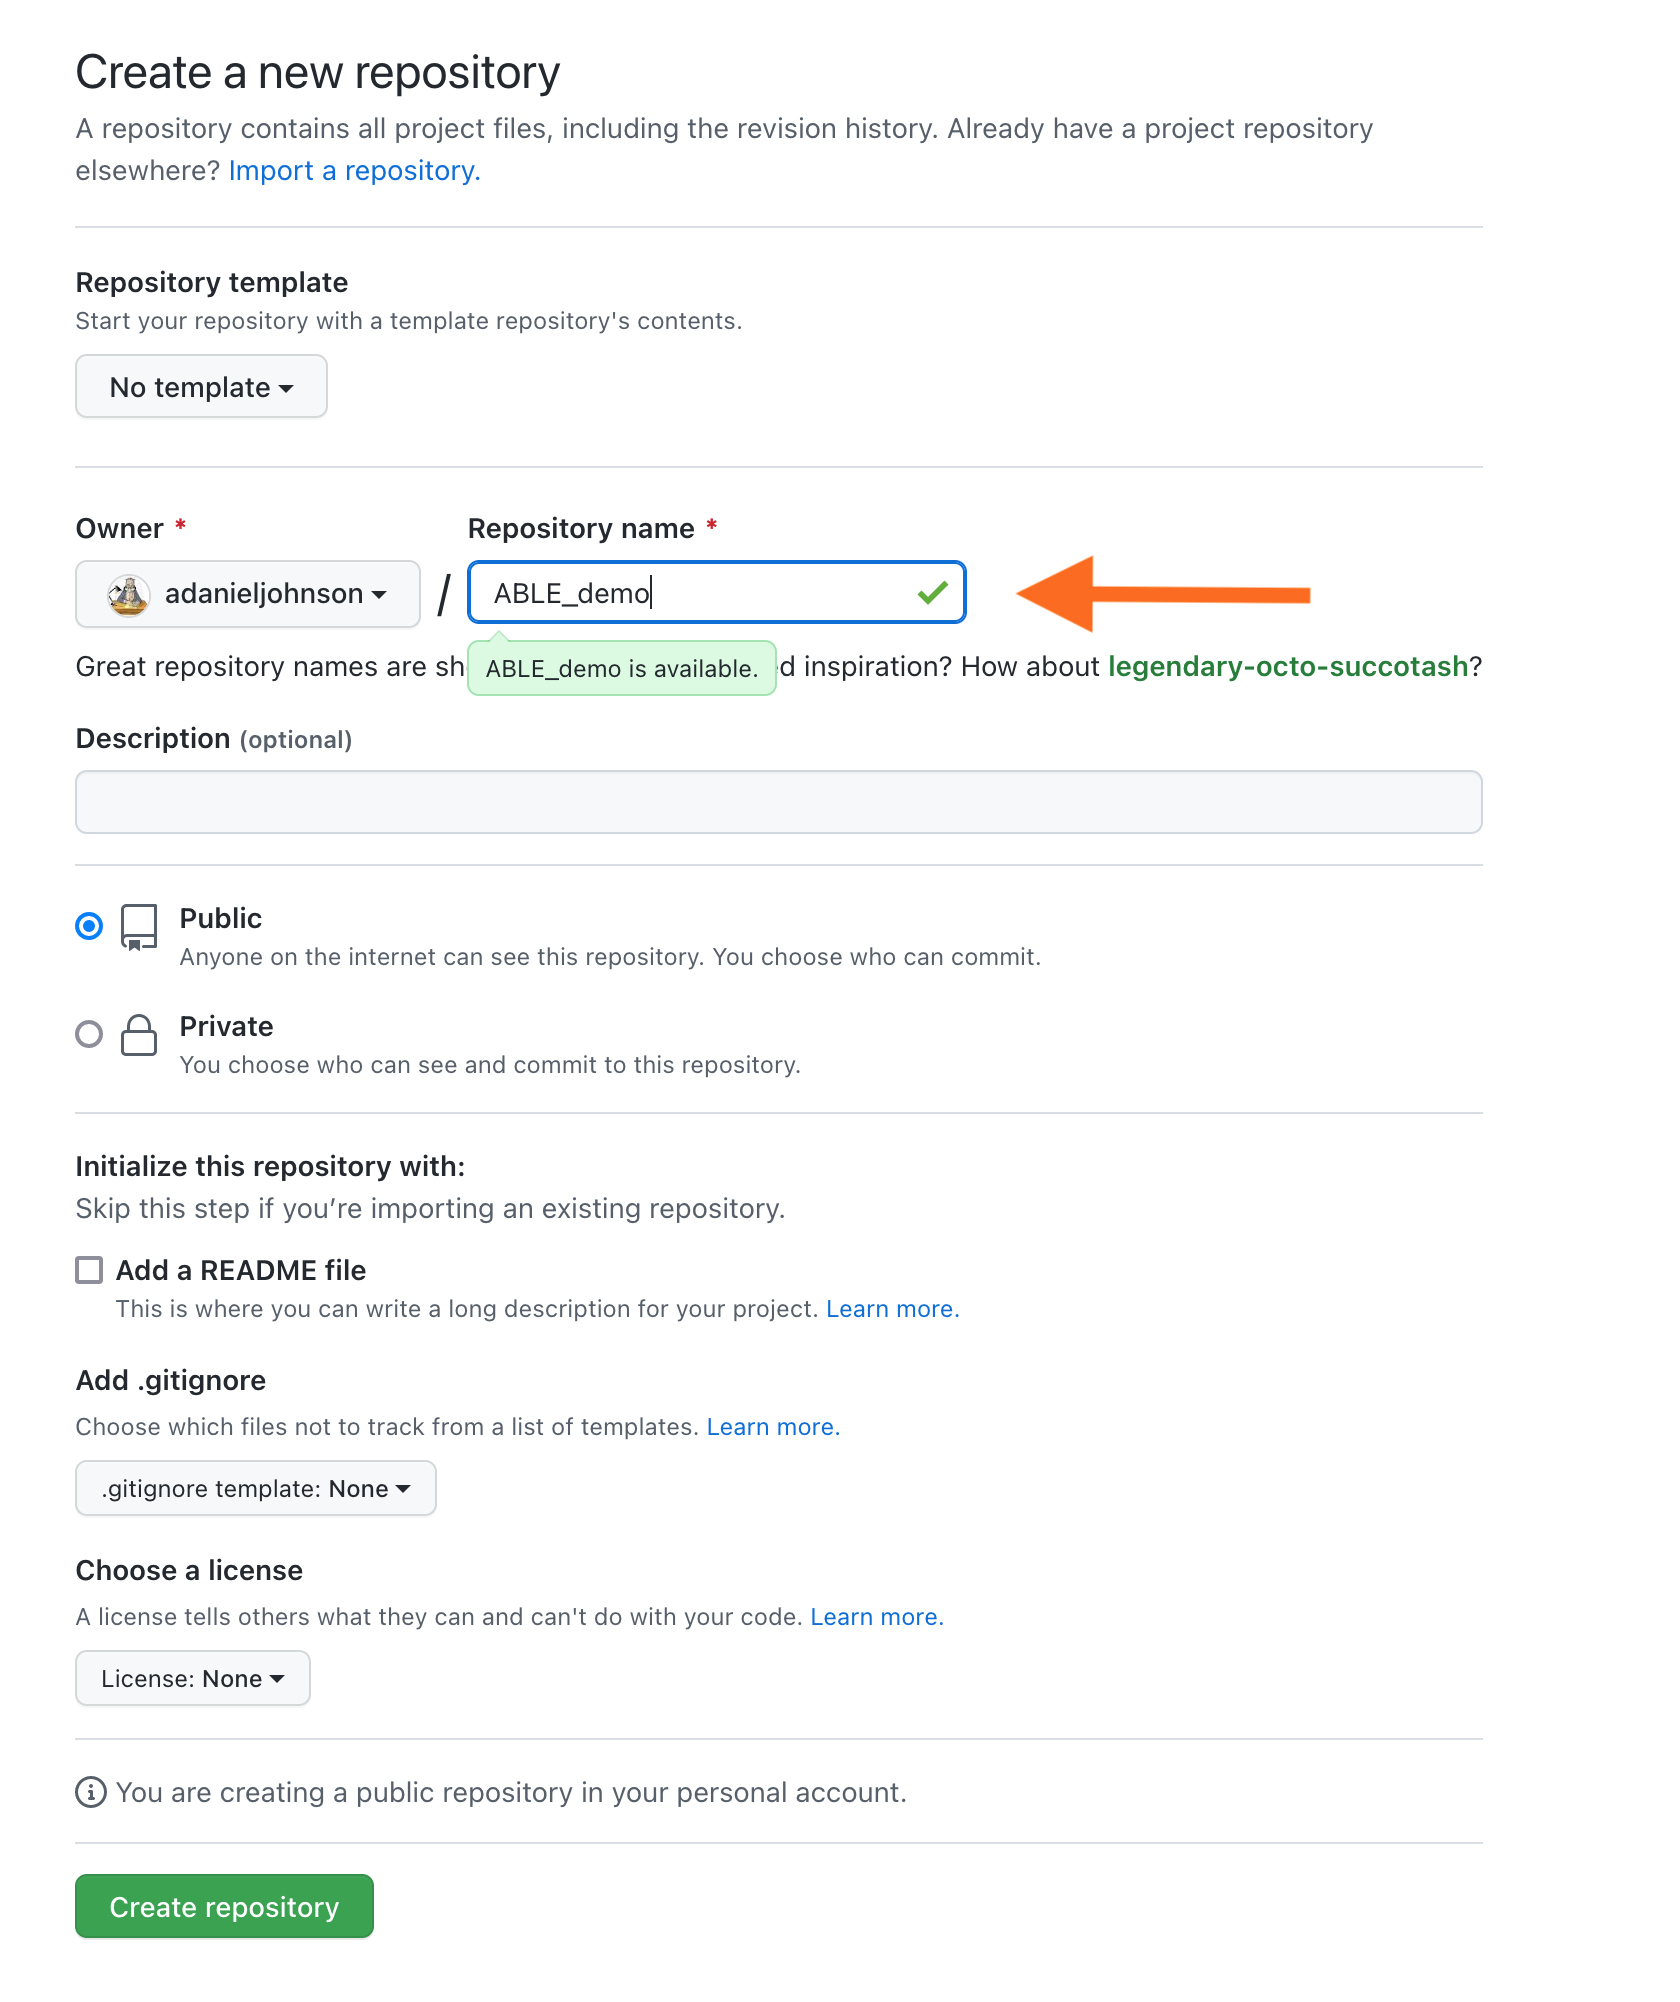
\includegraphics{https://github.com/adanieljohnson/ABLE_2022_Workshop/blob/main/images/Name_repo.png?raw=true}
\caption{Name your repo.}
\end{figure}

5. You will be asked to put files into the new repository. There are
several ways to add new files to a repository. You want to add
\textbf{existing} files.

\begin{figure}
\centering
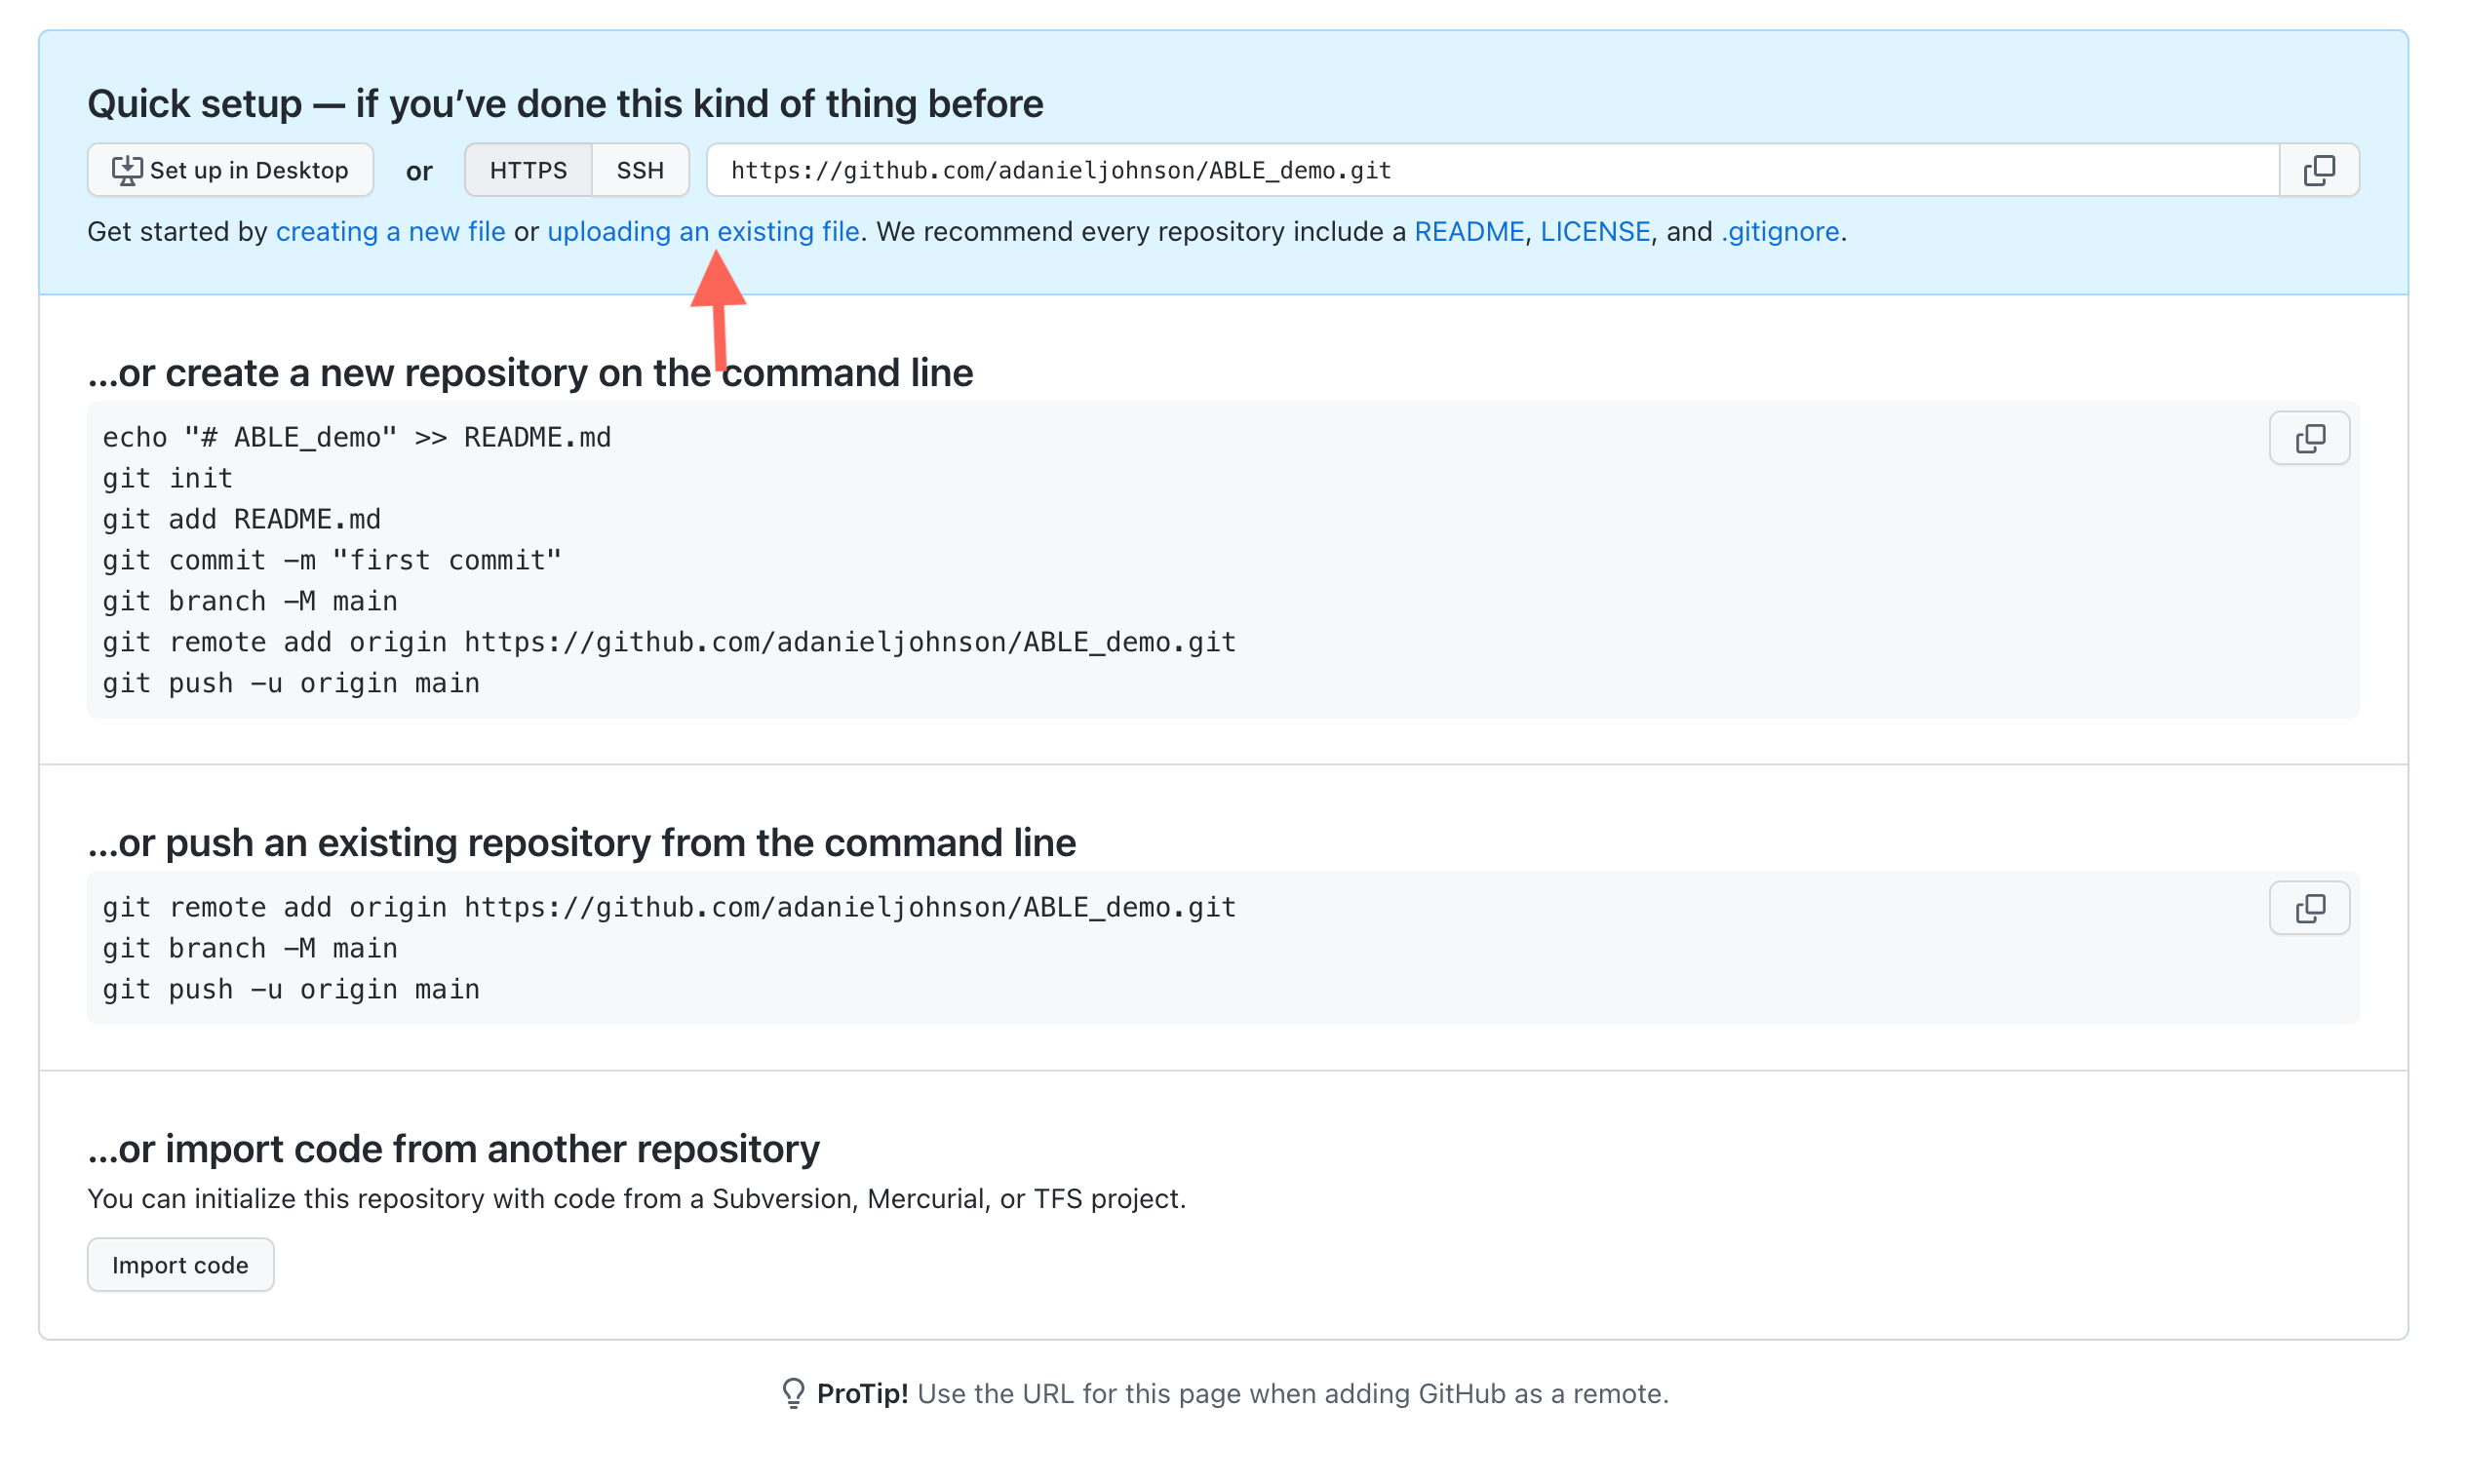
\includegraphics{https://github.com/adanieljohnson/ABLE_2022_Workshop/blob/main/images/Prep_repo.png?raw=true}
\caption{Preparing to add files.}
\end{figure}

6. In the dialog, drag in copies of 1-2 files that you have written
today.

\begin{figure}
\centering
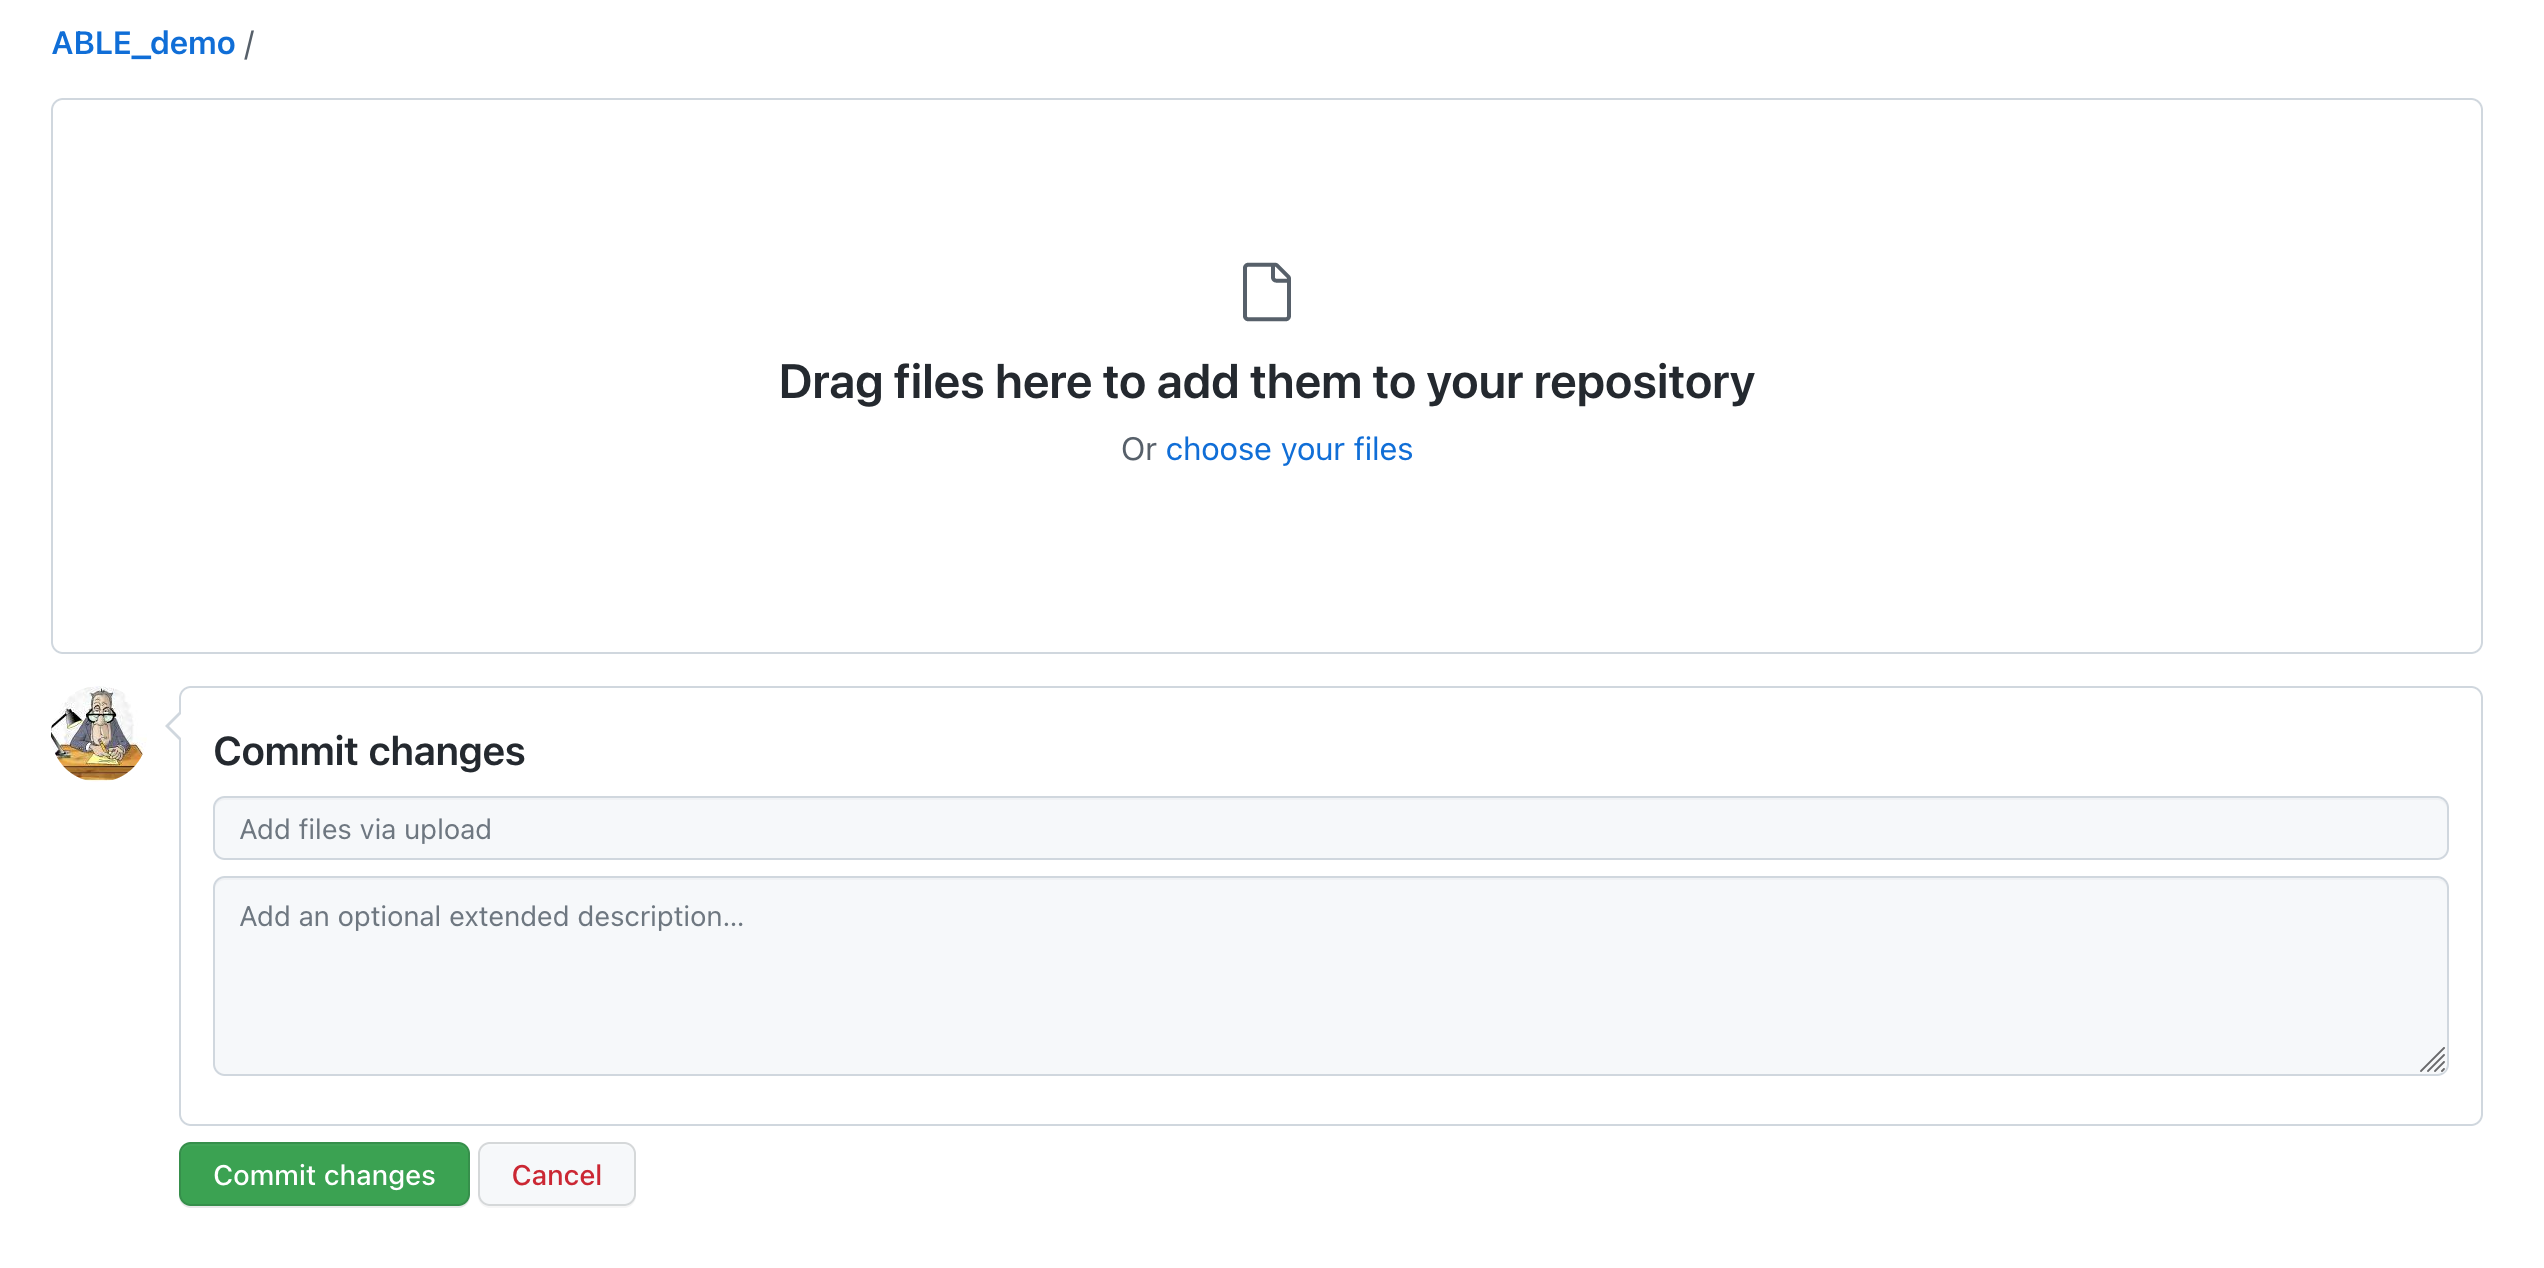
\includegraphics{https://github.com/adanieljohnson/ABLE_2022_Workshop/blob/main/images/Start_repo.png?raw=true}
\caption{Adding new files.}
\end{figure}

7. Take a look at your new repository. You should see the files you
added.

\begin{figure}
\centering
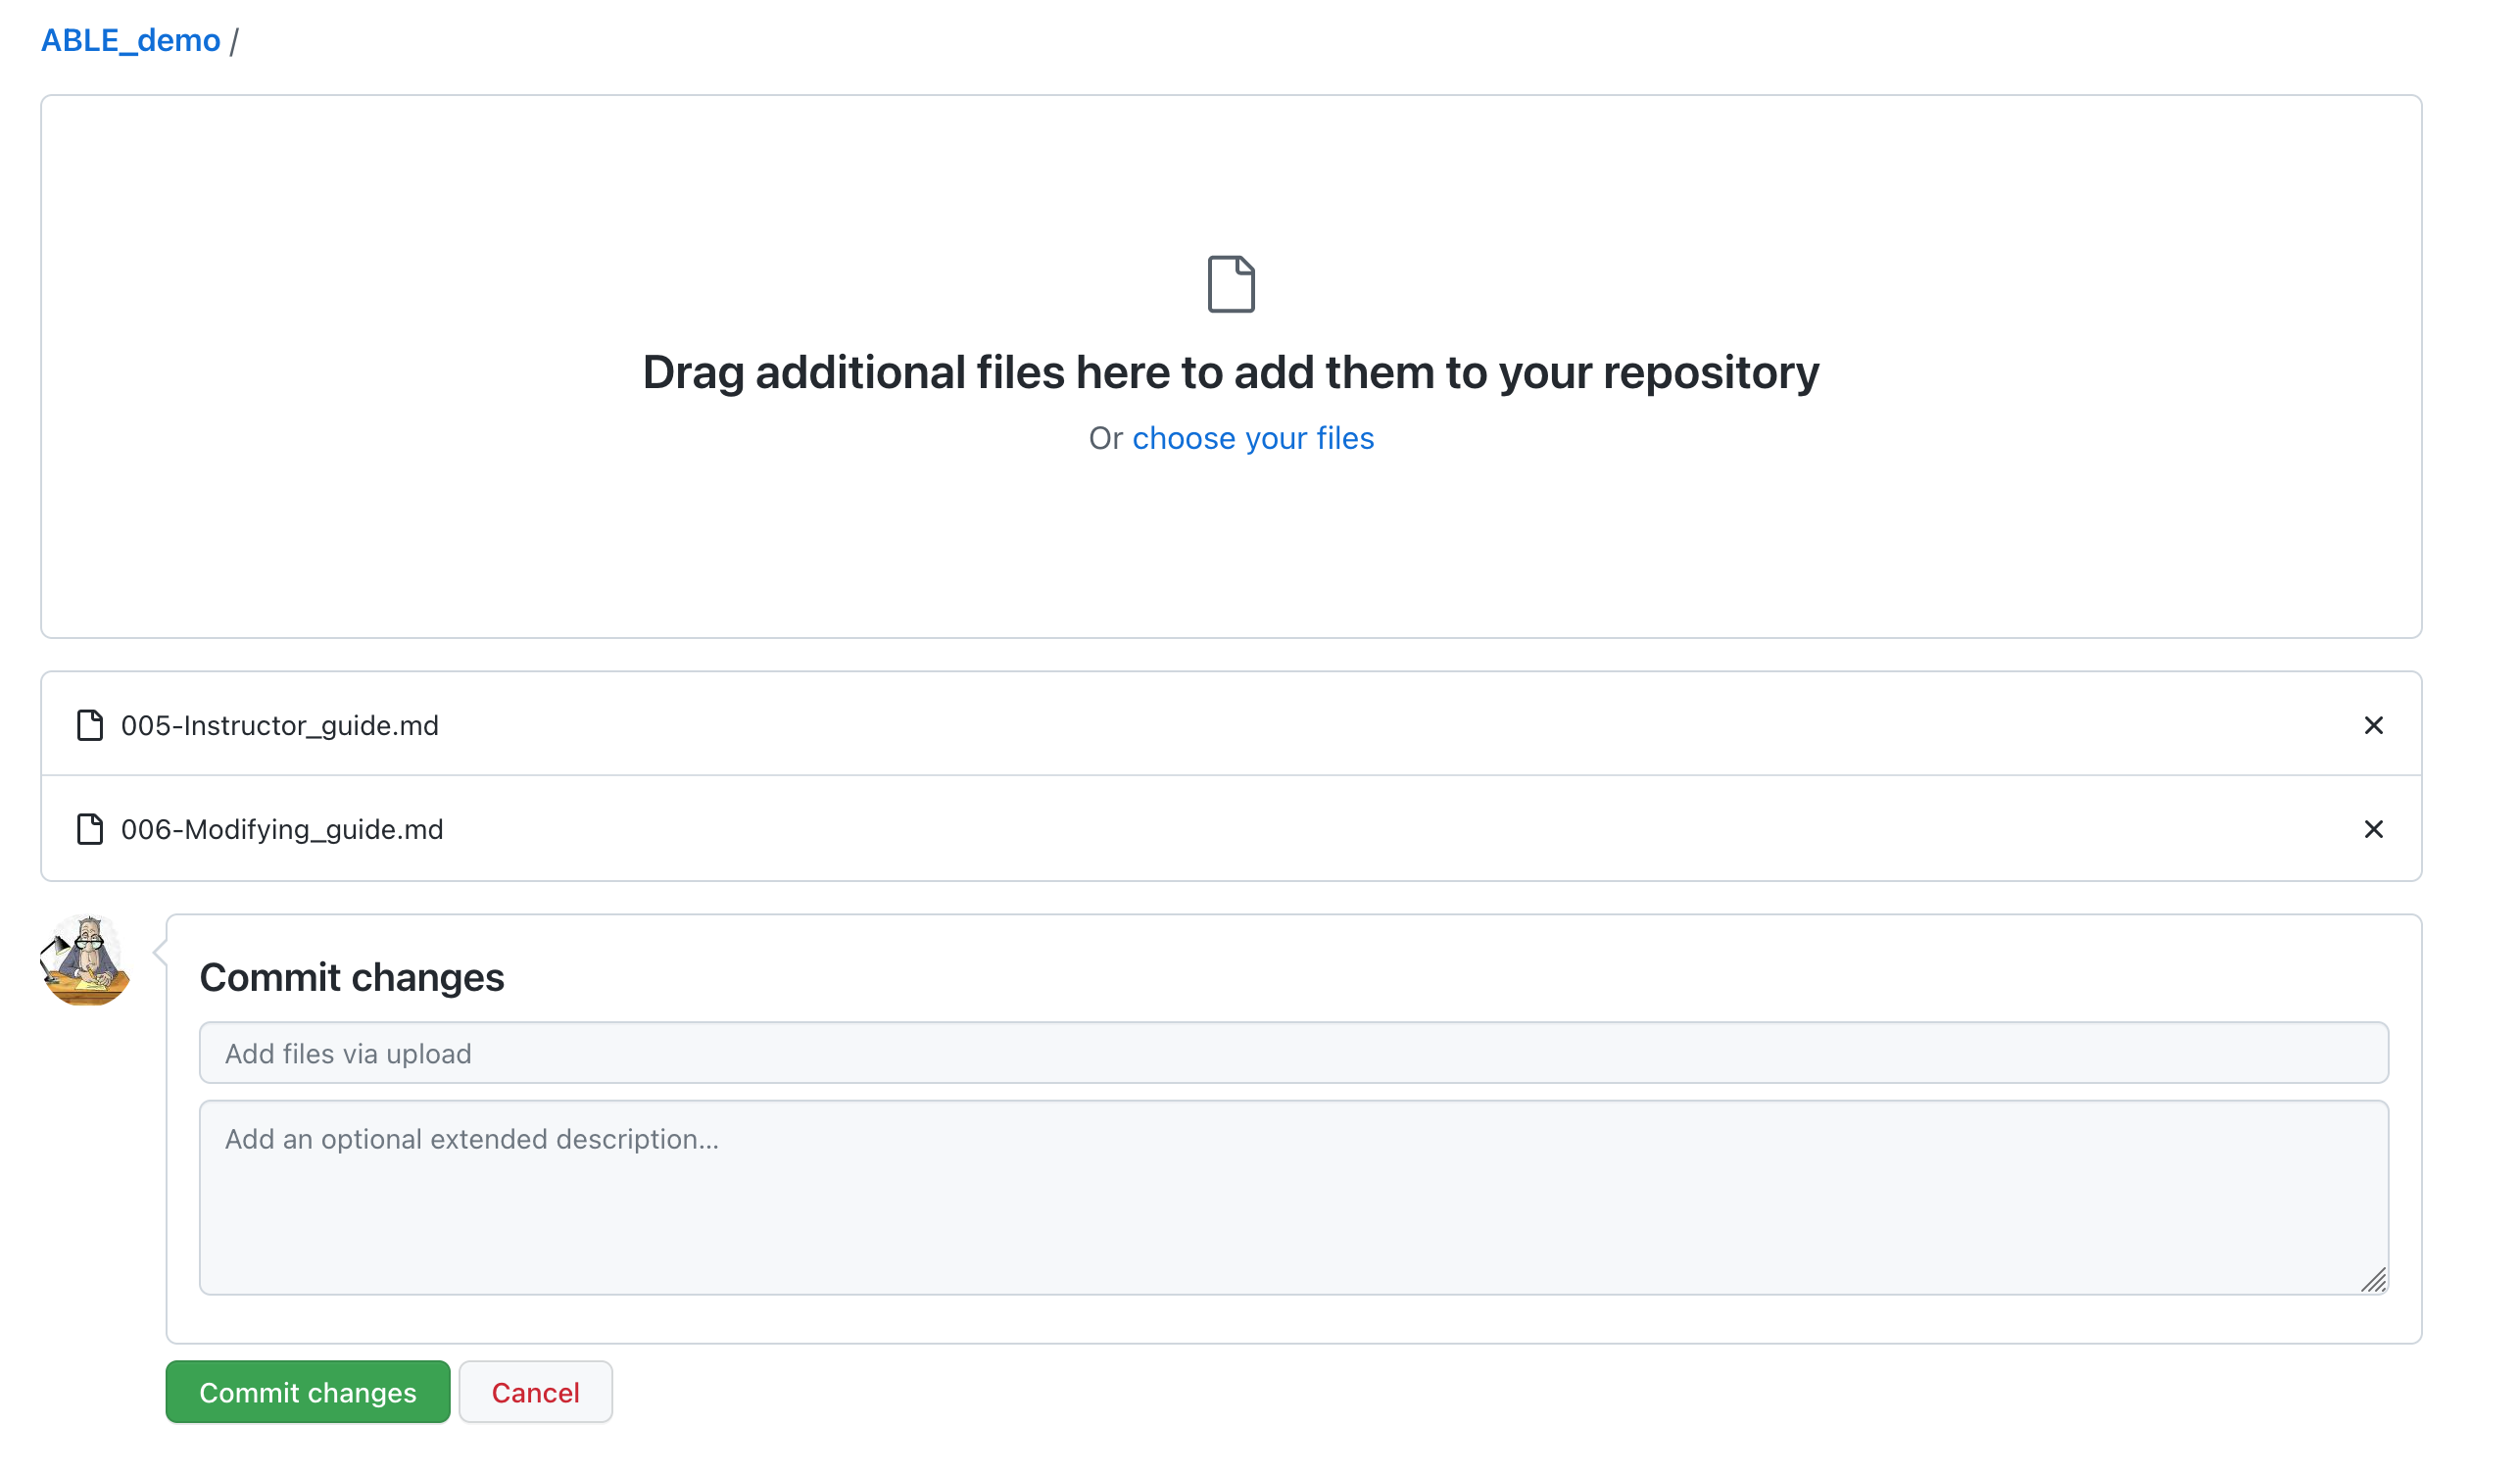
\includegraphics{https://github.com/adanieljohnson/ABLE_2022_Workshop/blob/main/images/Filled_repo.png?raw=true}
\caption{The first files in the new repo.}
\end{figure}

Next you will create a copy of this repo on your computer that is linked
to the version stored on GitHub.

8. Click on \textbf{Code}. You will see options for how to create a copy
of the new repo. Choose ``Open with GitHub Desktop.''

\begin{figure}
\centering
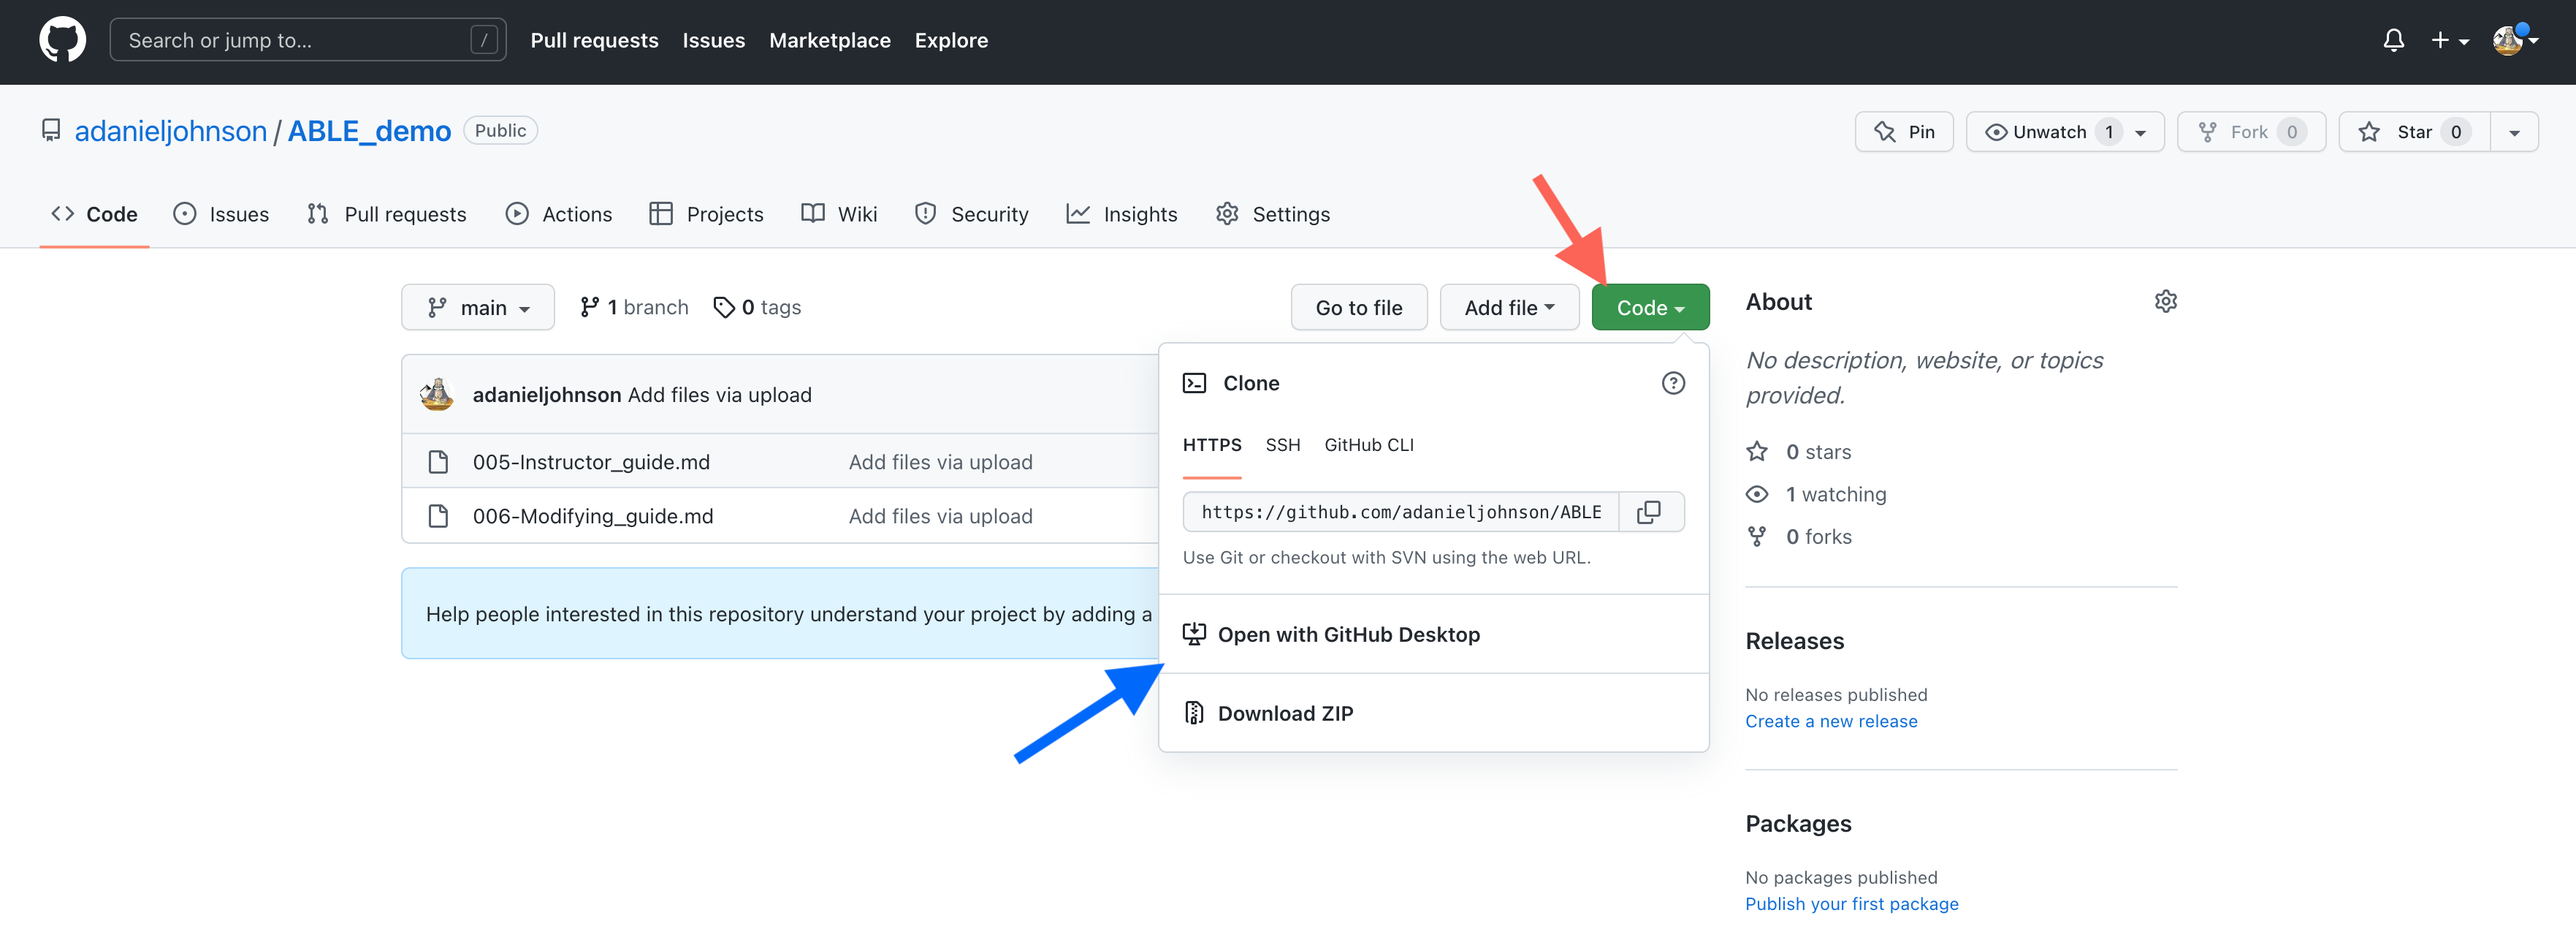
\includegraphics{https://github.com/adanieljohnson/ABLE_2022_Workshop/blob/main/images/Open_GH_desktop.png?raw=true}
\caption{Launching GitHub Desktop.}
\end{figure}

9. You will see a dialog that lets you set which folder will be
synchronized to GitHub. In practice, it usually is a good idea to put
repositories in a GitHub folder under Documents.

\begin{figure}
\centering
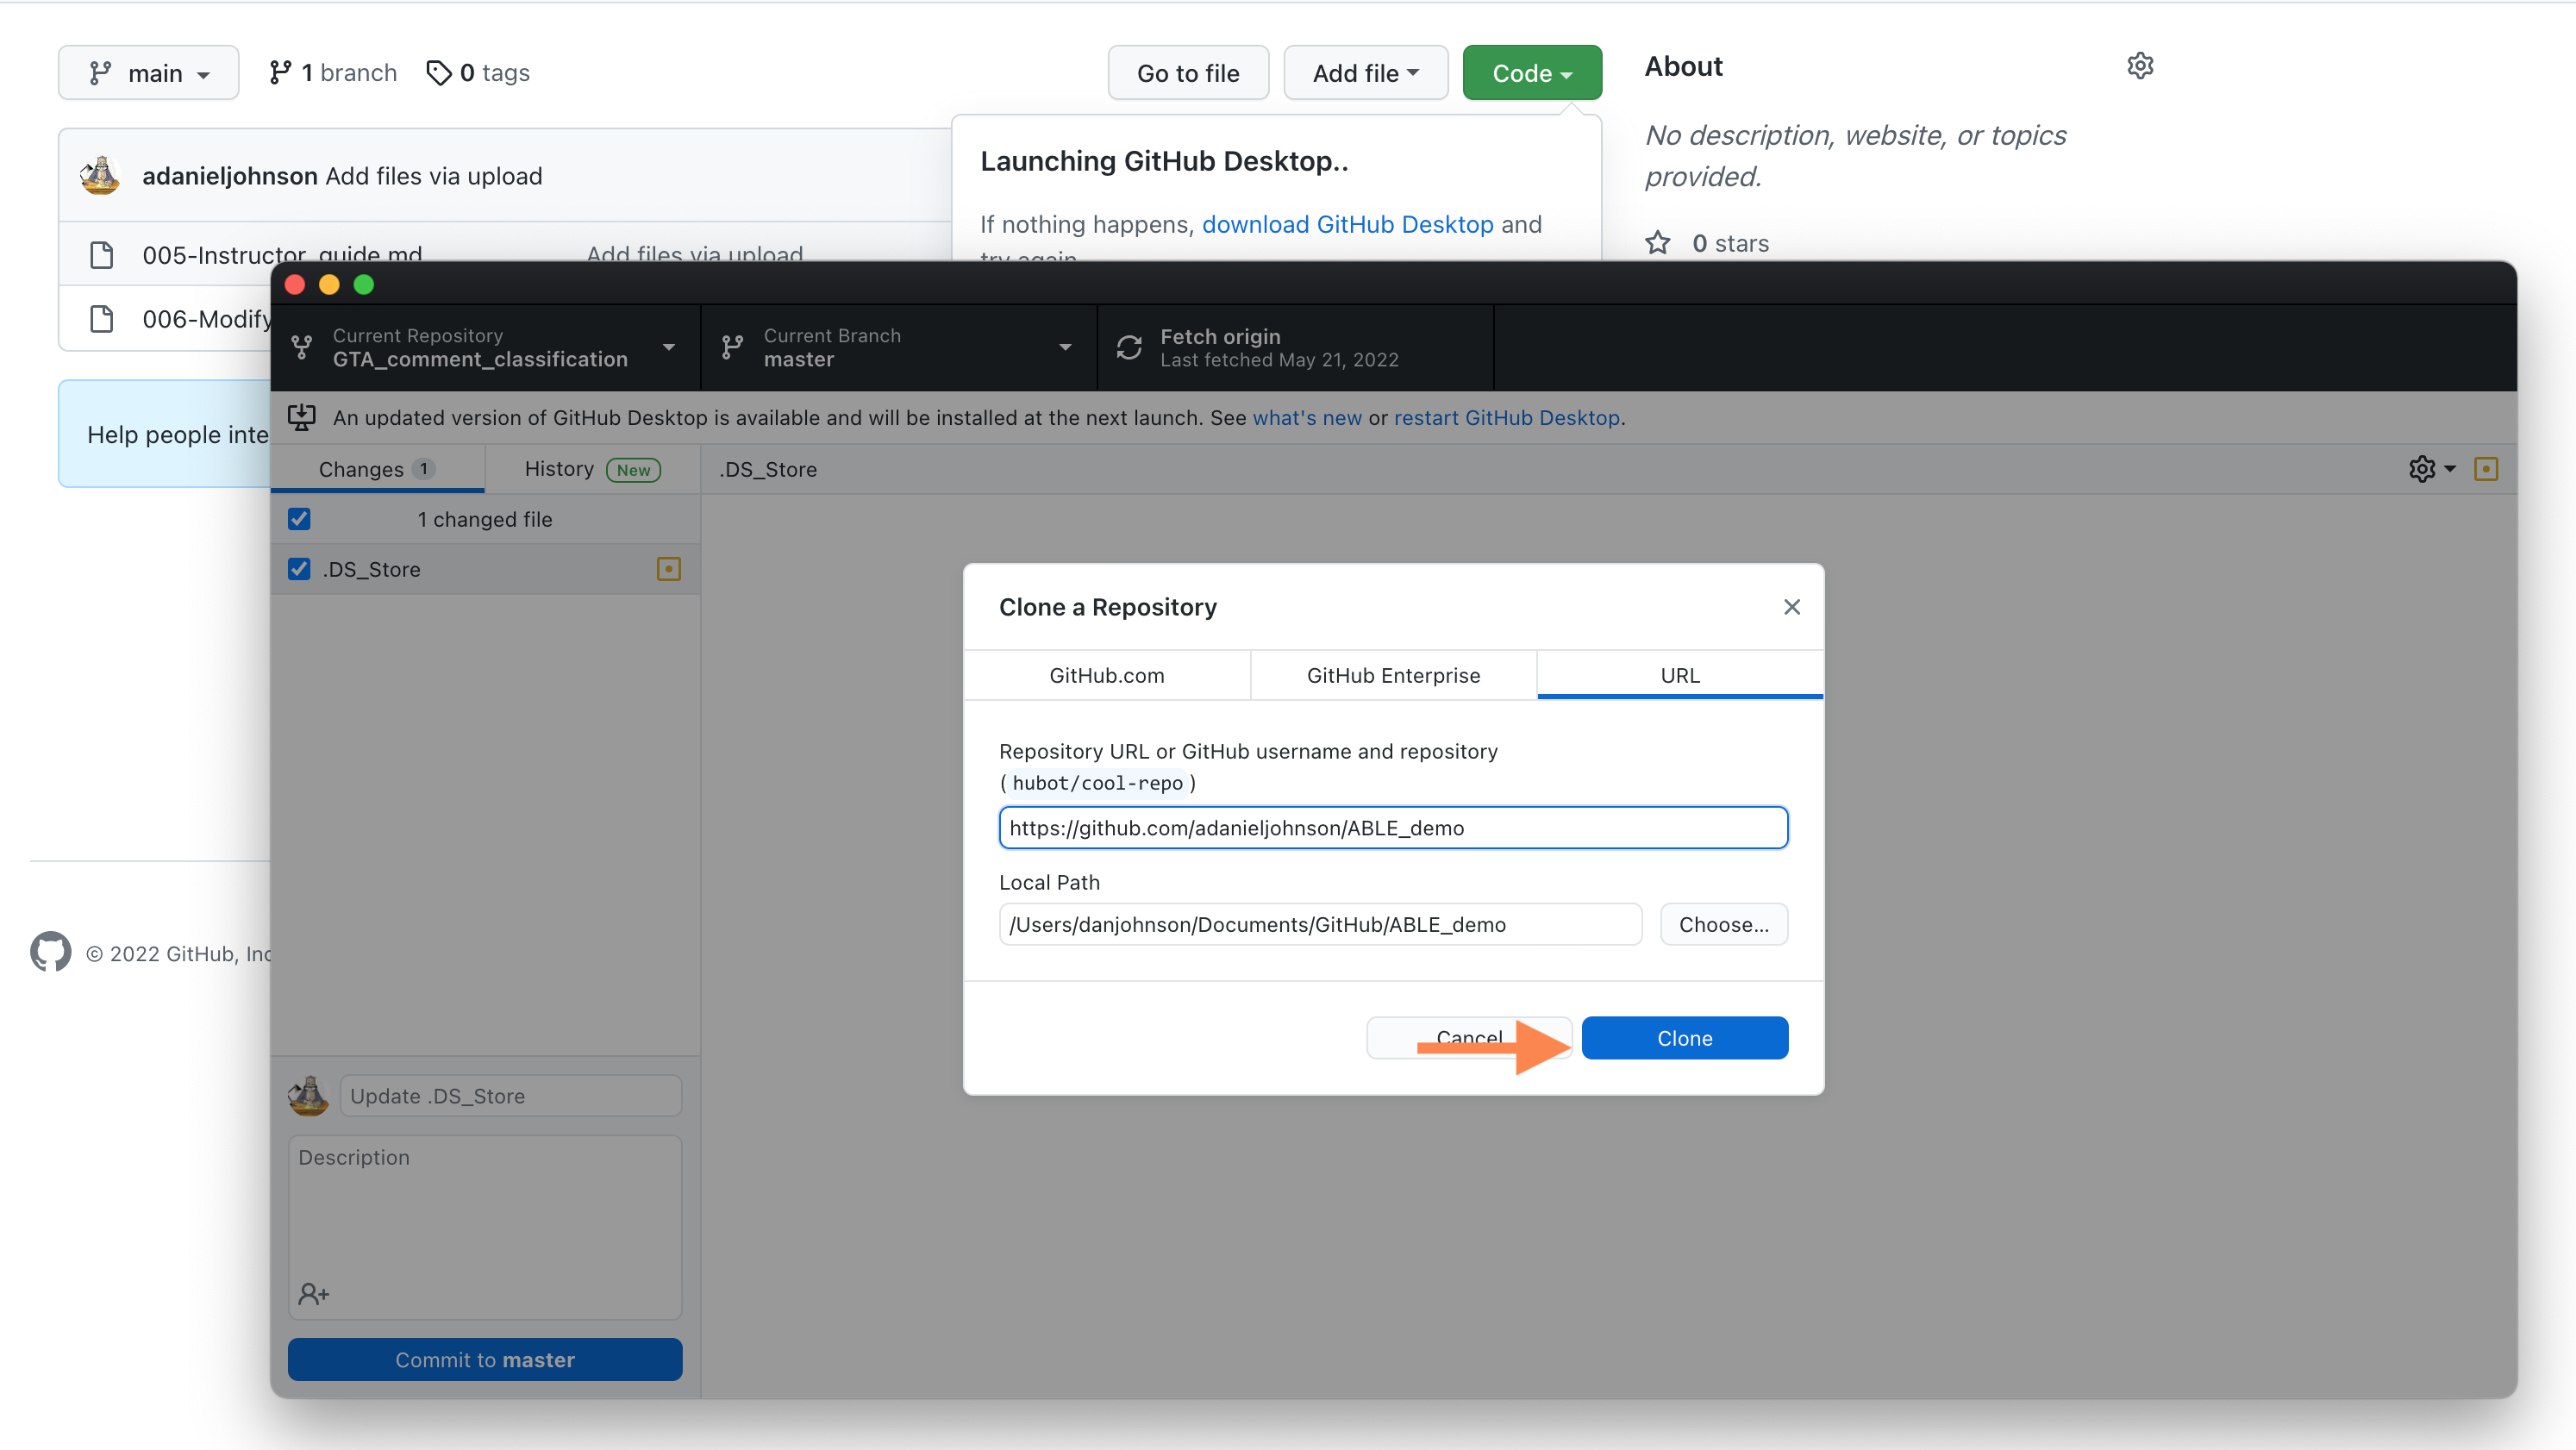
\includegraphics{https://github.com/adanieljohnson/ABLE_2022_Workshop/blob/main/images/Clone_locally.png?raw=true}
\caption{Dialog for creating a local copy of a GitHub repository.}
\end{figure}

10. After the cloned archive has been copied, you should be able to find
its folder on your local computer.

\begin{figure}
\centering
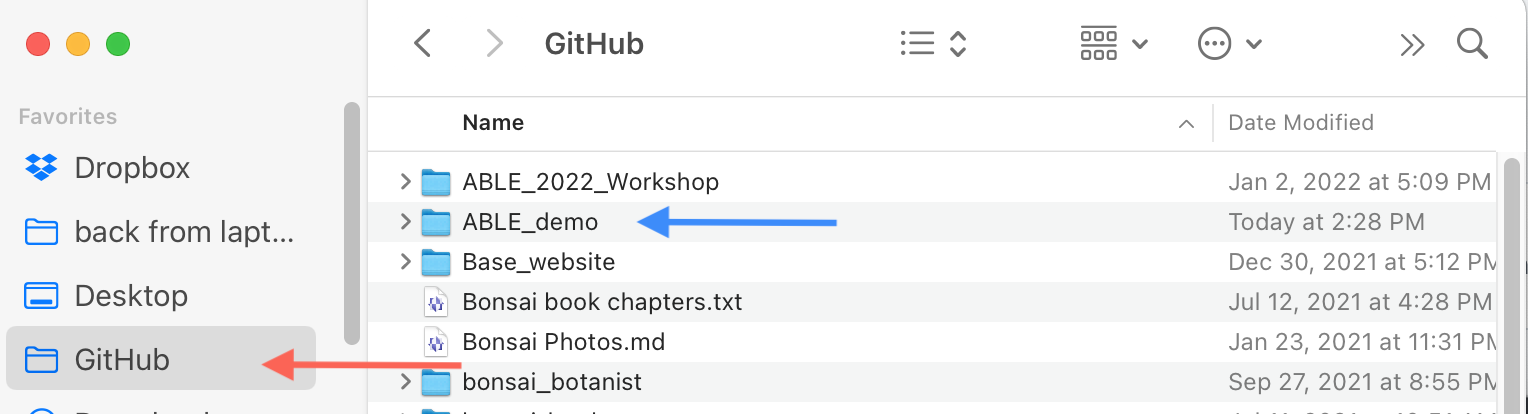
\includegraphics{https://github.com/adanieljohnson/ABLE_2022_Workshop/blob/main/images/Local_copy.png?raw=true}
\caption{In this example, ABLE\_demo repository (blue arrow) is stored
locally in a folder named ``GitHub.'' (orange arrow)}
\end{figure}

11. Each time you make a change in one or more local files, you need to
approve the changes (``commit'' them), then copy the changes (``push''
them) to the GitHub central server. GitHub Desktop helpfully shows you
what changes have been made to which files.

\begin{figure}
\centering
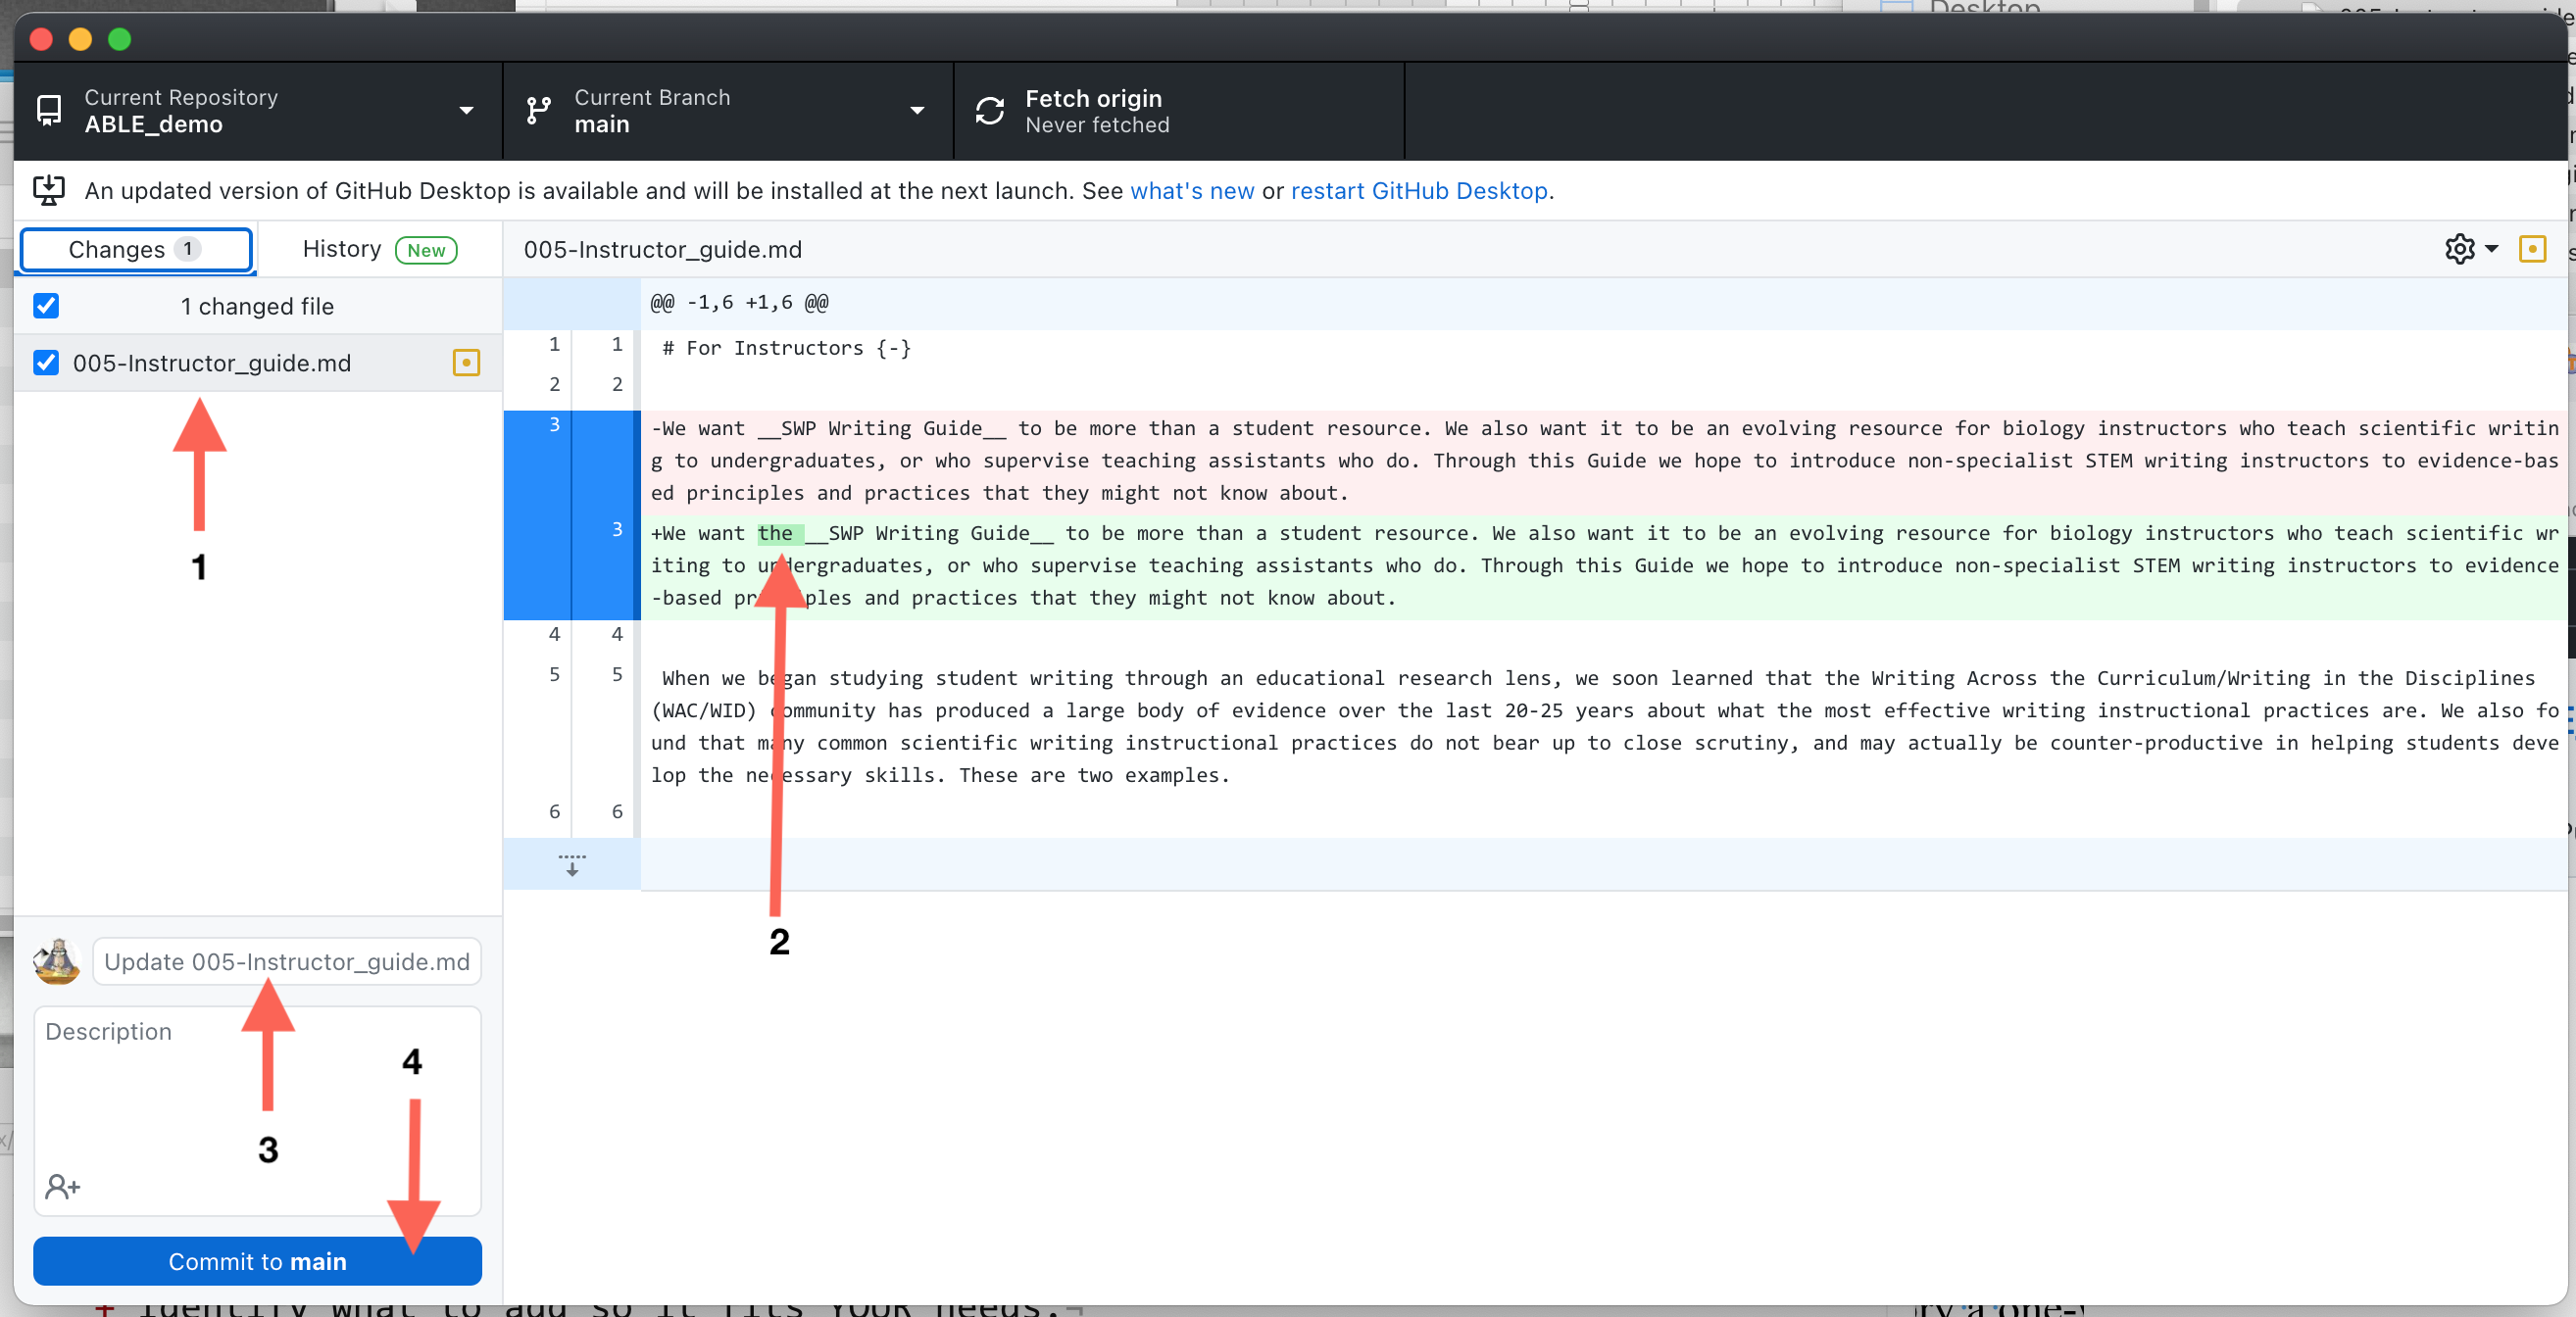
\includegraphics{https://github.com/adanieljohnson/ABLE_2022_Workshop/blob/main/images/Changes_log.png?raw=true}
\caption{How GitHub Desktop shows changes to files. Each file with a
change is listed (\#1) and the changes since the last version are
summarized (\#2). If you are updating one file the main change does not
have to be described (\#3) but if you are updating multiple files, you
need to give a short explanation of what you did. When you commit the
files (\#4) you are telling GitHub to update the copies on its main
server (\#4).}
\end{figure}

\begin{figure}
\centering
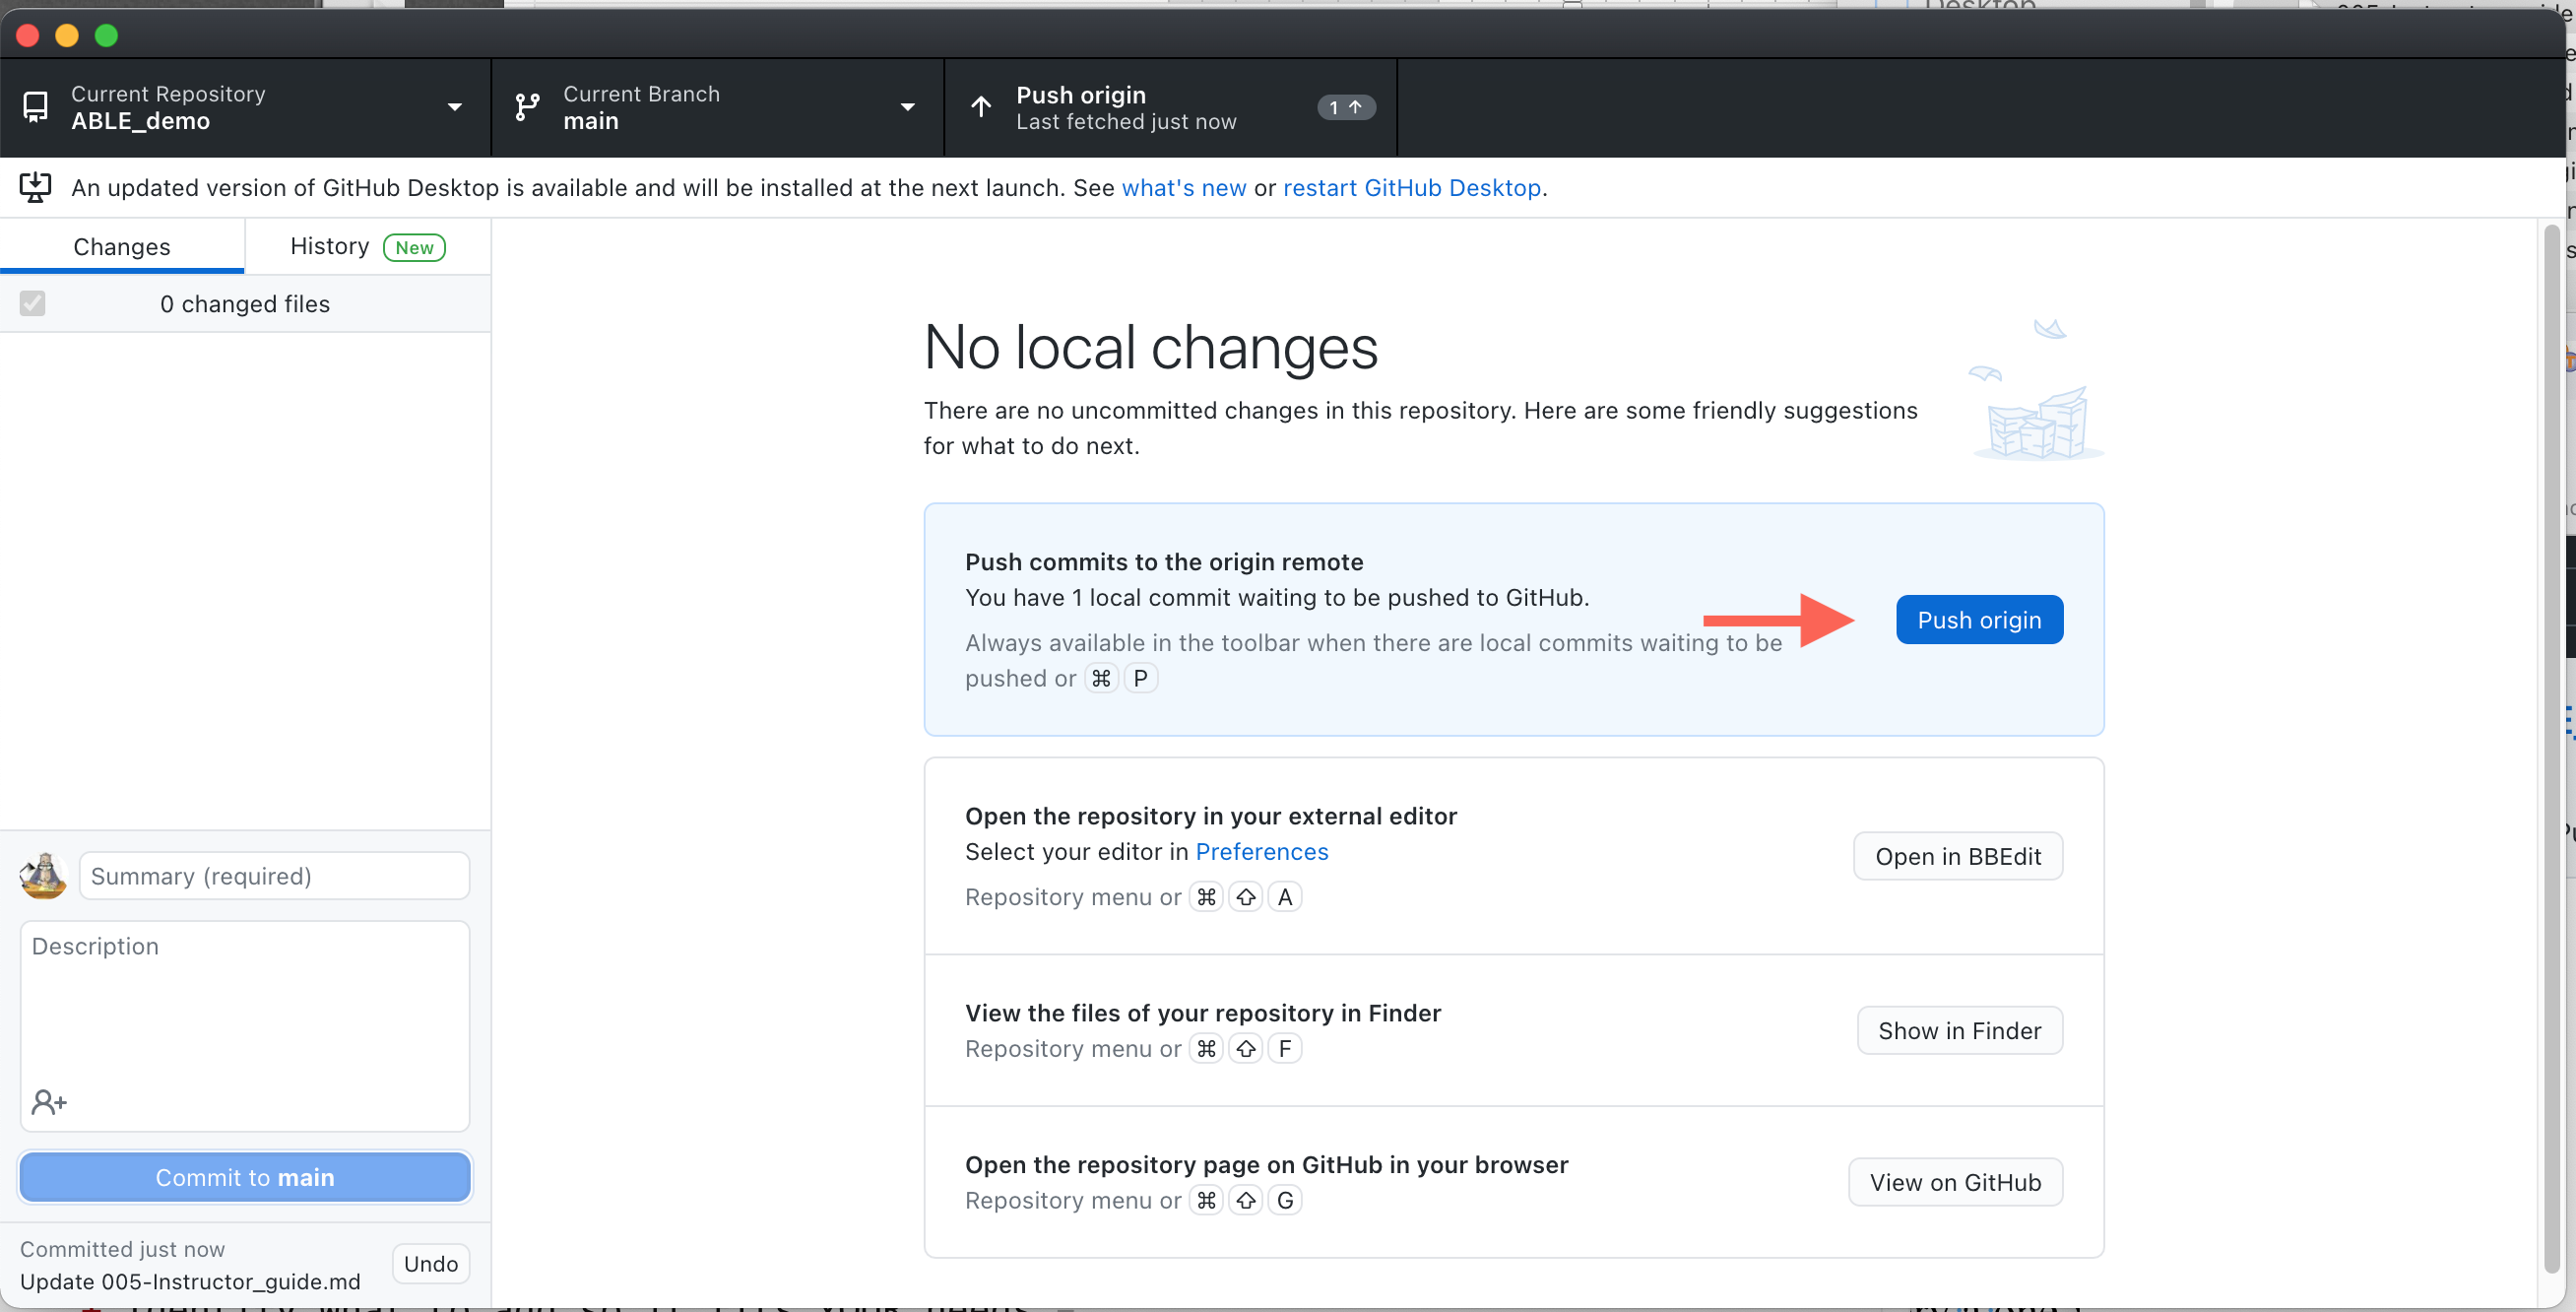
\includegraphics{https://github.com/adanieljohnson/ABLE_2022_Workshop/blob/main/images/Push_to_origin.png?raw=true}
\caption{Files are not updated on the GitHub central server until you
``Push'' them. Desktop shows changes to files. Each file with a change
is listed (\#1) and the changes since the last version are summarized
(\#2). If you are updating one file the main change does not have to be
described (\#3) but if you are updating multiple files, you need to give
a short explanation of what you did. When you commit the files (\#4) you
are telling GitHub to update the copies on its main server (\#4).}
\end{figure}

12. If you click on \textbf{Fetch Origin} again, you should get a
message saying \textbf{All files up to date}. This means your files in
the local copy and the server copy of the repository all match.

\hypertarget{tips-and-good-practices}{%
\subsubsection{Tips and Good Practices}\label{tips-and-good-practices}}

\textbf{How often should you commit and push?} It is up to you, but
generally you should commit every 30-60 minutes, or right after you
complete a set of major edits. You might only push changes to GitHub
once or twice a day, though more often does not hurt anything. It is a
good habit to push to GitHub when you finish working for the day.

\textbf{Why commit so often?} GitHub creates a detailed record of every
Commit and Push command in your account that includes which files were
changed and how. If you are editing a large file or several files and
accidentally delete some important text, you can use the repository
history to reconstruct the missing pieces. The more often you Commit,
the finer grained the record of changes.

\hypertarget{optional-writing-directly-inside-github}{%
\subsubsection{OPTIONAL: Writing Directly Inside
GitHub}\label{optional-writing-directly-inside-github}}

The workflow for creating and editing .md files in a browser is a bit
different than writing in R Studio or a text editor. These instructions
only work while you are online and logged into GitHub.

1. In a browser, log into GitHub (not Desktop). Go to the repository
containing your cloned copy of the Resource Guide. At the top of the
list, click on \textbf{Add file}. Choose \textbf{Create new file}.

2. Give your file a name that reflects the topic you did not see.
Include the .md extenstion.

3. Enter some starting text. One or two words is enough.

4. At the bottom of the page is the \textbf{Commit} dialog. GitHub
requires you to describe what you did when you save a file. That
information goes in the first box, and is required. It might seem like
extra trouble at first, but when you are making changes in critical
files, these commit comments can help you track what changes you made
and when. If there are multiple authors working on a file, each author's
changes should say specifically what they worked on.

5. Commit the file directly to the master (branches and pull requests
are not important until you are working on more complex projects.)
\textbf{TIP:} when you name files, do not include spaces. Write all file
names in CamelCase (FileName1.md) or Snake\_Case (File\_Name\_1.md)

6. Now you have a starting file that you can edit any way you wish. If
you want to see how changes to the Markdown code affect it, simply click
the \textbf{Preview} tab at the top of the window.

7. Next, go back to the Table of Contents and find a page you think you
might want to edit. Locate the corresponding pre-existing .md file, and
open it.

\begin{itemize}
\tightlist
\item
  First look at the current structure. If needed, compare it to the
  markup guide in Handout 3. Do you see how the structure of the
  rendered file is encoded in the Markdown tags? (Remember, click the
  \textbf{Preview} tab at the top of the window to switch from Code to
  Preview modes.)
\item
  Look for a section you want to edit. Make some changes, commit the
  file to your local repository, then see how your changes look using
  \textbf{Preview} mode.
\end{itemize}

\hypertarget{writing-tips-and-tricks-1}{%
\subsubsection{Writing Tips and
Tricks}\label{writing-tips-and-tricks-1}}

\begin{itemize}
\tightlist
\item
  Always start Markdown pages with a Level 1 header that is the title of
  the document. Reserve the Level 1 header just for that purpose. This
  does not seem very useful at first, but it becomes essential when you
  start compiling multiple .md files into longer documents or books.
\item
  It is tempting to remove spaces between lines of text in .md files.
  BAD idea! Markdown relies on blank lines to keep track of blocks of
  text. When Markdown is rendered, extra blank lines are deleted
  automatically.
\item
  When editing inside GitHub or a text editor, pages may extend beyond
  the screen. If so, for a drop-down or setting in the Preferences that
  says \textbf{Soft wrap}. This keeps sentences and paragraphs from
  running off the right side of the screen.
\end{itemize}

\hypertarget{next-steps}{%
\section{Next Steps}\label{next-steps}}

Today's exercises introduced you to most of the tools you need to start
using Markdown.

If you want to use our Writing Resource Guide in your own courses, you
now have the original documents and all the tools you need to edit it to
suit your program needs. If you are interested in writing new material
or helping us expand the Guide, let us know.

If you want to try building your own online book, go to our
\href{https://github.com/adanieljohnson/bookdown-demo}{Bookdown Demo}
repository, which is an unmodified fork of a demo by bookdown's creator,
Yihui Yue. Clone this to a new repository, and you have a complete
operating skeleton for a book.
\href{https://bookdown.org/yihui/bookdown/}{Authoring Books and
Technical Documents With R Markdown} describes how to customize it as
you desire.

Two other books that can help you continue developing your skills are:

\begin{itemize}
\tightlist
\item
  \href{https://bookdown.org/yihui/bookdown/}{Guide to using Bookdown}
\item
  \href{https://bookdown.org/yihui/rmarkdown/}{Using Markdown inside R}
\end{itemize}

\hypertarget{links-to-resources}{%
\section{Links to Resources}\label{links-to-resources}}

Links to packages and resources described in the workshop handouts are
provided again here for convenience, along with additional resources.

\hypertarget{getting-started}{%
\subsubsection{Getting Started}\label{getting-started}}

\begin{itemize}
\tightlist
\item
  \href{https://www.portent.com/blog/content/content-with-github-markdown.htm}{WHY
  and HOW to write well-structured, reusable texts}
\item
  \href{https://github.com/adanieljohnson/ABLE_2022_Workshop}{Workshop
  Repository and Writing Resource Guide}
\end{itemize}

\hypertarget{free-plain-text-editors}{%
\subsubsection{Free Plain Text Editors}\label{free-plain-text-editors}}

\begin{itemize}
\tightlist
\item
  \href{https://texteditor.co/}{Google Text Editor} is available to
  anyone with a Gmail account. It is not as full-featured as many
  editors, but does recognize Markdown natively.
\item
  Microsoft's \href{https://code.visualstudio.com/}{Visual Code Studio}
  is a very powerful open-source text and code editor. It comes with
  support for Markdown files right out of the box. The main drawback is
  that some commands are where you think they should be.
\item
  \href{https://brackets.io/}{Brackets} is popular with many code and
  text wranglers. It displays Markdown but does not export it easily.
\end{itemize}

\hypertarget{markdown-native-editors}{%
\subsubsection{Markdown-Native Editors}\label{markdown-native-editors}}

\begin{itemize}
\tightlist
\item
  \href{https://notepad-plus-plus.org/}{Notepad++} is the default
  installed text editor for Windows. The
  \href{https://github.com/nea/MarkdownViewerPlusPlus}{MarkdownViewer++
  plugin} adds the ability to render and export Markdown contents to
  HTML. Detailed instructions for installing the MDV++ plugin are
  available
  \href{https://adamtheautomator.com/convert-markdown-to-html/}{here},
  and
  \href{https://techwombat.com/how-to-install-markdownviewer-plus-plus-plugin-notepad-plus-plus/}{here}.
\item
  \href{http://pad.haroopress.com/}{HarooPad} produces very clean HTML.
\item
  \href{https://stackedit.io/}{StackEdit} integrates with Dropbox,
  Google Drive, and other online services. A good choice if you mostly
  work with HTML, and need tight integration with Google Drive.
\end{itemize}

\hypertarget{using-github}{%
\subsubsection{Using GitHub}\label{using-github}}

\begin{itemize}
\tightlist
\item
  \href{https://desktop.github.com/}{Install GitHub Desktop}
\item
  \href{https://github.com/}{GitHub home page}
\item
  \href{https://docs.github.com/en/desktop/installing-and-configuring-github-desktop/overview/getting-started-with-github-desktop}{Getting
  Started With GitHub Desktop}
\end{itemize}

\hypertarget{markdown-syntax-and-add-ons}{%
\subsubsection{Markdown Syntax and
Add-Ons}\label{markdown-syntax-and-add-ons}}

\begin{itemize}
\tightlist
\item
  \href{https://docs.github.com/en/github/writing-on-github/getting-started-with-writing-and-formatting-on-github/basic-writing-and-formatting-syntax}{GitHub's
  Introduction to GHFM}
\item
  \href{https://guides.github.com/features/mastering-markdown/}{Quick
  Guide to Mastering Markdown}
  *\href{https://www.markdownguide.org/extended-syntax/}{Extended Syntax
  for Markdown}
\item
  \href{https://github.com/ikatyang/emoji-cheat-sheet/blob/master/README.md}{Emoji
  cheat sheet}. There are two ways to add emoji to Markdown files: copy
  and paste an emoji into the Markdown-formatted text, or type emoji
  shortcodes. GHFM does not support emoji shortcodes, so copy/paste from
  this cheat sheet is your best option.
\item
  \href{https://www.pluralsight.com/guides/working-tables-github-markdown}{Making
  Tables in Markdown}
\item
  \href{https://www.tablesgenerator.com/markdown_tables}{Web-based
  Markdown Table Maker}
\item
  \href{https://www.w3schools.com/html/html_formatting.asp}{HTML
  shortcuts}
\item
  \href{https://www.w3schools.com/html/html_symbols.asp}{HTML special
  symbols}
\item
  \href{https://www.overleaf.com/learn/latex/Mathematical_expressions}{Writing
  LaTeX equations}
\item
  \href{https://latex.codecogs.com/legacy/eqneditor/editor.php}{Online
  equation builder}
\item
  \href{https://github.github.com/gfm/}{Official Specification for
  GHFM}, if you want to see the complete documentation.
\end{itemize}

\hypertarget{file-format-converters}{%
\subsubsection{File Format Converters}\label{file-format-converters}}

\begin{itemize}
\tightlist
\item
  HTML5 for the web:

  \begin{itemize}
  \tightlist
  \item
    \href{https://ashkanph.github.io/md-to-html/}{MD to HTML Converter}
  \item
    \href{https://dillinger.io/}{Dillinger}
  \item
    \href{https://markdown-it.github.io/}{Markdown It}
  \item
    \href{https://markdowntohtml.com/}{Markdown to HTML}
  \end{itemize}
\item
  MS Word documents:

  \begin{itemize}
  \tightlist
  \item
    \href{https://pandoc.org/demos.html}{Pandoc Converter}
  \end{itemize}
\end{itemize}

\hypertarget{r-and-r-studio-bookdown-package}{%
\subsubsection{R and R Studio; Bookdown
Package}\label{r-and-r-studio-bookdown-package}}

\begin{itemize}
\tightlist
\item
  \href{https://cloud.r-project.org/}{Install R}.
\item
  \href{https://www.rstudio.com/products/rstudio/download/}{Install
  RStudio}.
\item
  \href{https://moderndive.netlify.app/1-getting-started.html}{Installing
  R and R Studio, Step by Step}
\item
  \href{https://bookdown.org/yihui/rmarkdown/}{Using Markdown inside R}
\item
  \href{https://bookdown.org/}{Home page for the R Bookdown package}
\item
  \href{https://bookdown.org/yihui/bookdown/}{Guide to using Bookdown}
\end{itemize}

\hypertarget{commercial-products}{%
\subsubsection{Commercial Products}\label{commercial-products}}

\begin{itemize}
\tightlist
\item
  \href{https://marked2app.com/}{Marked 2} is an inexpensive desktop
  application for previewing Markdown. Mac only.
\item
  \href{http://markdownpad.com/}{Markdown Pad} is similar to Marked 2,
  but for Windows.
\item
  \href{https://typora.io/}{Typora} lets you write and view Markdown
  immediately. Costs \$15. Works well for Word documents, but adds extra
  code to HTML.
\item
  \href{https://caret.io/}{Caret} is a newer cross-platform tool.
\end{itemize}

\hypertarget{workshop-debrief}{%
\section{Workshop Debrief}\label{workshop-debrief}}

At the end of the workshop we will talk about three of the original
goals of this workshop, what we learned, and what can be improved.

\hypertarget{goal-1.-introduce-the-biology-writing-resource-guide}{%
\subsubsection{Goal 1. Introduce the Biology Writing Resource
Guide}\label{goal-1.-introduce-the-biology-writing-resource-guide}}

We want the Resource Guide to be widely useful.

\begin{enumerate}
\def\labelenumi{\arabic{enumi}.}
\tightlist
\item
  What other pages are needed?
\item
  What other resources would be helpful?
\item
  Do you have resources you would like to contribute?
\end{enumerate}

\hypertarget{goal-2.-introduce-markdown-supporting-tools}{%
\subsubsection{Goal 2. Introduce Markdown, supporting
tools}\label{goal-2.-introduce-markdown-supporting-tools}}

We plan to train others to modify the Resource Guide.

\begin{enumerate}
\def\labelenumi{\arabic{enumi}.}
\tightlist
\item
  What other training materials would be helpful?
\item
  What should we add, remove from training?
\end{enumerate}

\hypertarget{goal-3.-expand-experiment-with-our-workshop-model}{%
\subsubsection{Goal 3. Expand, experiment with our workshop
model}\label{goal-3.-expand-experiment-with-our-workshop-model}}

If someone must switch suddenly to a Zoom format, what can they do to
make it better?

\begin{enumerate}
\def\labelenumi{\arabic{enumi}.}
\tightlist
\item
  What works well? (Ex. mixed teams, varied presentation, episodic work
  w/reporting)
\item
  What needs improvement? What could be added?
\item
  Does having a local helper make it easier?
\end{enumerate}

\end{document}
